\chapter{Instantiating a cognitive model for driving context classification}
\label{chap:driving_context_classification}

In this chapter, we describe the first application task or our driving scene representation based on semantic vectors: the classification of the current driving context.
We use the tools of the \ac{SPA} and the representation approaches shown in section~\ref{subsec:structured_representations} to generate semantic vectors describing the current scene.
Given this representation of the driving situation, we aim to classify the current driving context, i.e., if we are currently driving on a highway, in a city or on an interurban road.
We have already discussed in section~\ref{subsec:driving_context_classification}, that high-accuracy digital maps could be used in combination with the vehicle's current position measured using \ac{SensGPS} to detect the driving context, which is probably the most accurate approach to driving context classification.
However, inferring contextual information from on-board sensory data is appealing as either a fallback option in situations when \ac{SensGPS} is not available of if keeping an updated map with driving context information is not feasible.
Furthermore, it is an interesting option and a good candidate to firstly investigate our vector representation for automotive scenes, as it seems to be a moderately complex task in the context of automated driving, yet still challenging enough, since we need to combine symbol-like processing with numerical data.

Fig.~\ref{subfig:system_overview_horizontal} shows a schematic overview of our approach to driving context classification  and the general flow of information within the system.
Environment perception happens through the ego-vehicle's on-board sensors such as cameras, \ac{RADAR} and \ac{LIDAR} sensors providing data either in the form of either already preprocessed object-lists or unprocessed raw sensory data.
From this data, we generate our vector representation encapsulating the structure and semantics of the current scene, which will be used as input for the classification system.
In the subsequent sections, we will describe the data sets used for driving context classification alongside the preprocessing steps performed to prepare the data for the task at hand, our vector representation for the current driving scene and the models used for classifying the current driving context.
Finally, we will evaluate the systems performance and compare it to two performance baselines.
In the evaluation stage, we will also investigate the influence of variations in the vocabulary of atomic vectors on the performance of the classification system.

\section{Data and preprocessing}%
\label{sec:data_and_preprocessing_context_classification}

The input data used for training and evaluating the driving context classification models is real-world data gathered during test drives in the region of Munich, Germany.
Depending on the test vehicle's sensor setup \parencite{Aeberhard2015}, a subset of the following extrospective sensor systems is available: cameras, \ac{RADAR} and \ac{LIDAR} sensors.
Furthermore, the dynamics of the ego-vehicle such as velocity, acceleration or the steering angle are measured using introspective sensors.
While all extrospective sensors provide preprocessed lists of dynamic objects such as cars or pedestrians, the camera system additionally detects static objects such as traffic signs.
Furthermore, the raw images of both, the front and rear camera are also available. 

In this chapter, we focus on the ego-vehicle's dynamics and the information provided by the camera-system as the only extrospective sensor, since there are no object-lists with information fused from several sensor sources available.
Furthermore, the camera-system is present in all available test traces and its data is most informative regarding categories of dynamic objects while being the only system that provides information about traffic signs.
The camera provides class labels for each object such as \emph{car} or \emph{pedestrian} for dynamic objects as well as the type of each detected traffic sign.
Apart from these object classification labels, the camera sensor provides estimations for other object features such as position and orientation relative to the ego-vehicle and furthermore dynamic information such as velocity or acceleration for moving objects only.
We divide the available data into a training and a test set, which contain roughly \SI{27}{\minute} and \SI{18}{\minute} of driving data respectively.

\subsection{Data labeling}%
\label{subsec:data_labeling}

\begin{figure}[t]
    \centering
    \subfloat[\label{subfig:context_class_city_end_interurban_start_img}]{%
        \includegraphics[width=0.5\linewidth]{imgs/context_class_city_end_interurban_start_img.png}
    }
    \subfloat[\label{subfig:context_class_highway_start}]{%
        \includegraphics[width=0.5\linewidth]{imgs/context_class_highway_start.png}
    }
    \caption{Two example images illustrating a change of the current driving context as indicated by~\protect\subref{subfig:context_class_city_end_interurban_start_img} a traffic sign marking the exit of city and~\protect\subref{subfig:context_class_highway_start} a traffic sign marking the entrance to a highway.
    The traffic signs are highlighted by a red rectangle.}
    \label{fig:context_class_manual_labeling}
\end{figure}

To enable automated training of any supervised learning system, the training data needs to be labeled. 
Since there is no labeled data set publicly available neither was the driving data labeled regarding the current driving context, we had to label our own data set.
In this chapter, we focus on three driving context labels only, namely \emph{city}, \emph{interurban} and \emph{highway}.
Hence, the goal is to assign one of these labels to all data points in our driving data set.
We achieved this goal by manually labeling the driving context by inspecting the images provided by the ego-vehicle's on-board camera systems.
To avoid including human bias into the labeling regarding what sorts of situations belong to each of the labels, we restricted the labeling process to finding traffic signs indicating a change of driving context and assign the respective labels to all data points between these context switches.
Figure~\ref{fig:context_class_manual_labeling} shows two example situations where the ego-vehicle transitions from one driving context to another, namely from city driving to interurban driving as indicated by the city exit traffic sign in Fig.~\ref{subfig:context_class_city_end_interurban_start_img} and from interurban context to highway driving as indicated by the highway entrance traffic sign in Fig.~\ref{subfig:context_class_highway_start}.
This manual labeling process yields \SIlist{53.6;18.9;27.5}{\percent} of the samples in the training set belonging to \emph{city}, \emph{interurban} and \emph{highway} driving respectively while \SIlist{23.3;5;25.9}{\percent} of the samples in the test set belong to the same driving context labels.

\section{Representation and models}%
\label{sec:representation_and_modelsi_context_classification}

In this section, we describe our approach to encode driving situations in semantic vectors to classify the current driving context from them.
We present the different types of information we encode in the vector representation using several underlying vocabularies to evaluate their impact on the model classification performance.
Finally, we describe the models trained to produce the actual context classification.

\subsection{Scene representation in vectors}%
\label{subsec:scene_representation_in_vectors_context_classification}
\begin{figure}[t]
    \centering
    \resizebox{.9\textwidth}{!}{%
        \subfloat[\label{subfig:Example_scene}]{%
            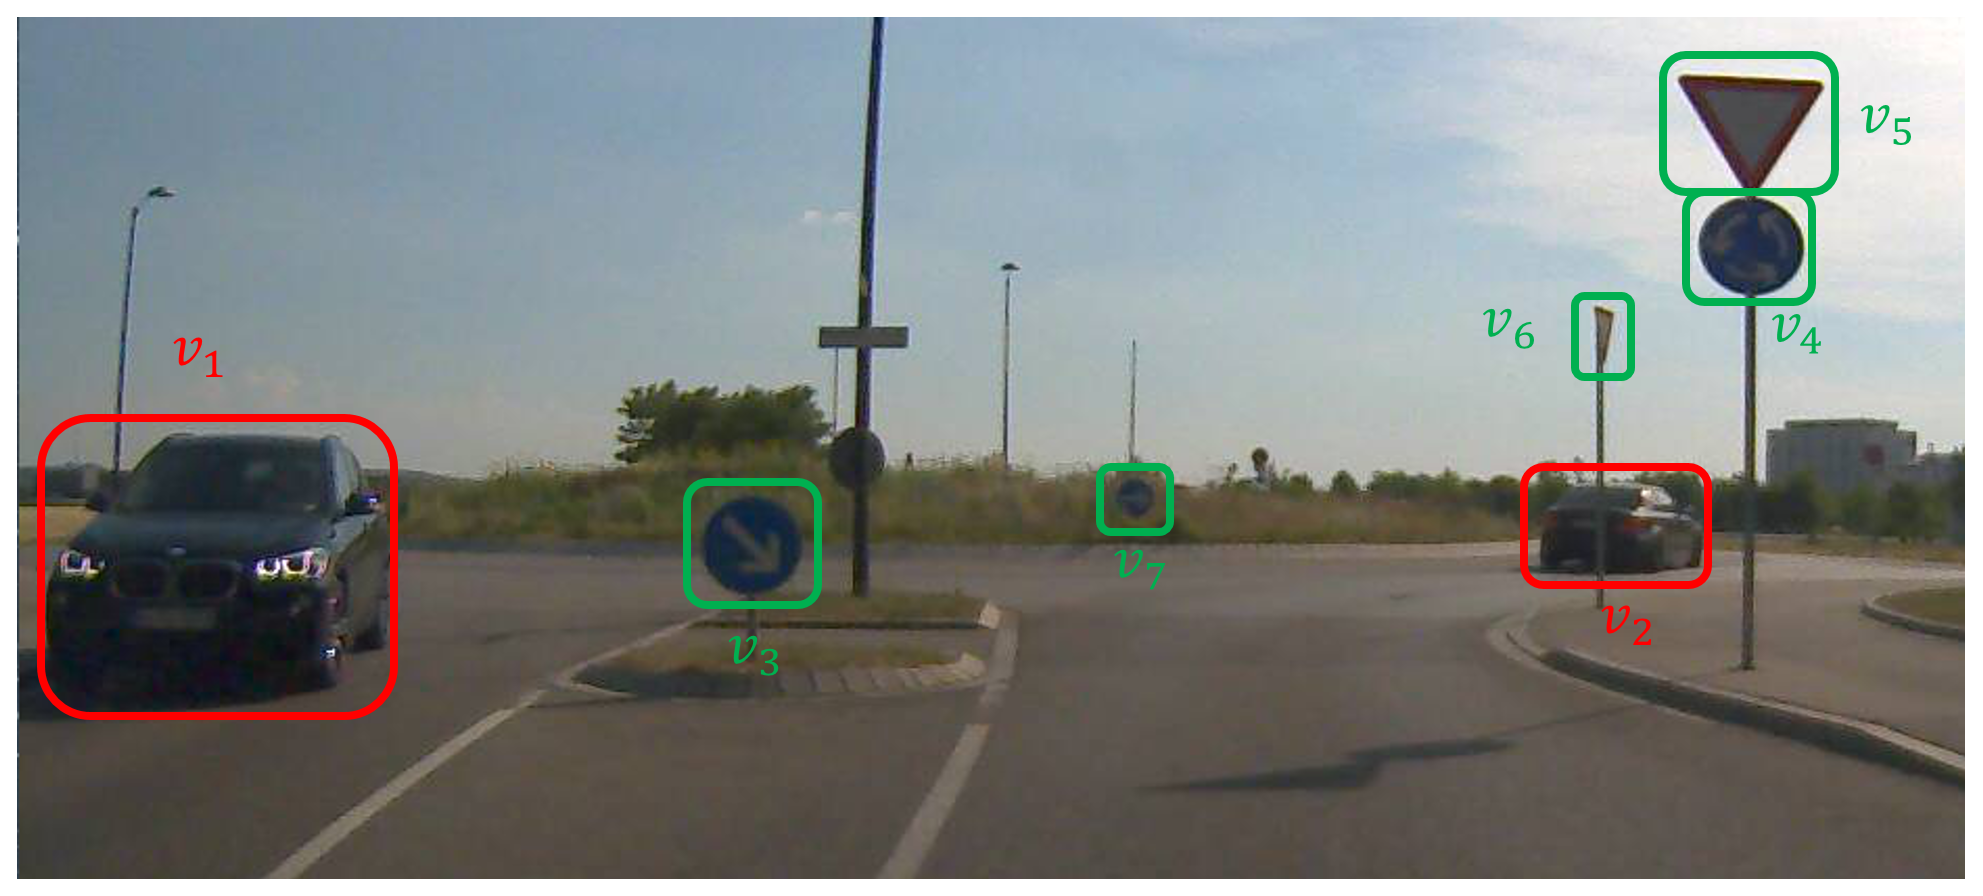
\includegraphics[height=3cm]{imgs/Example_scene.eps}
        }
        \subfloat[\label{subfig:system_overview_horizontal}]{%
            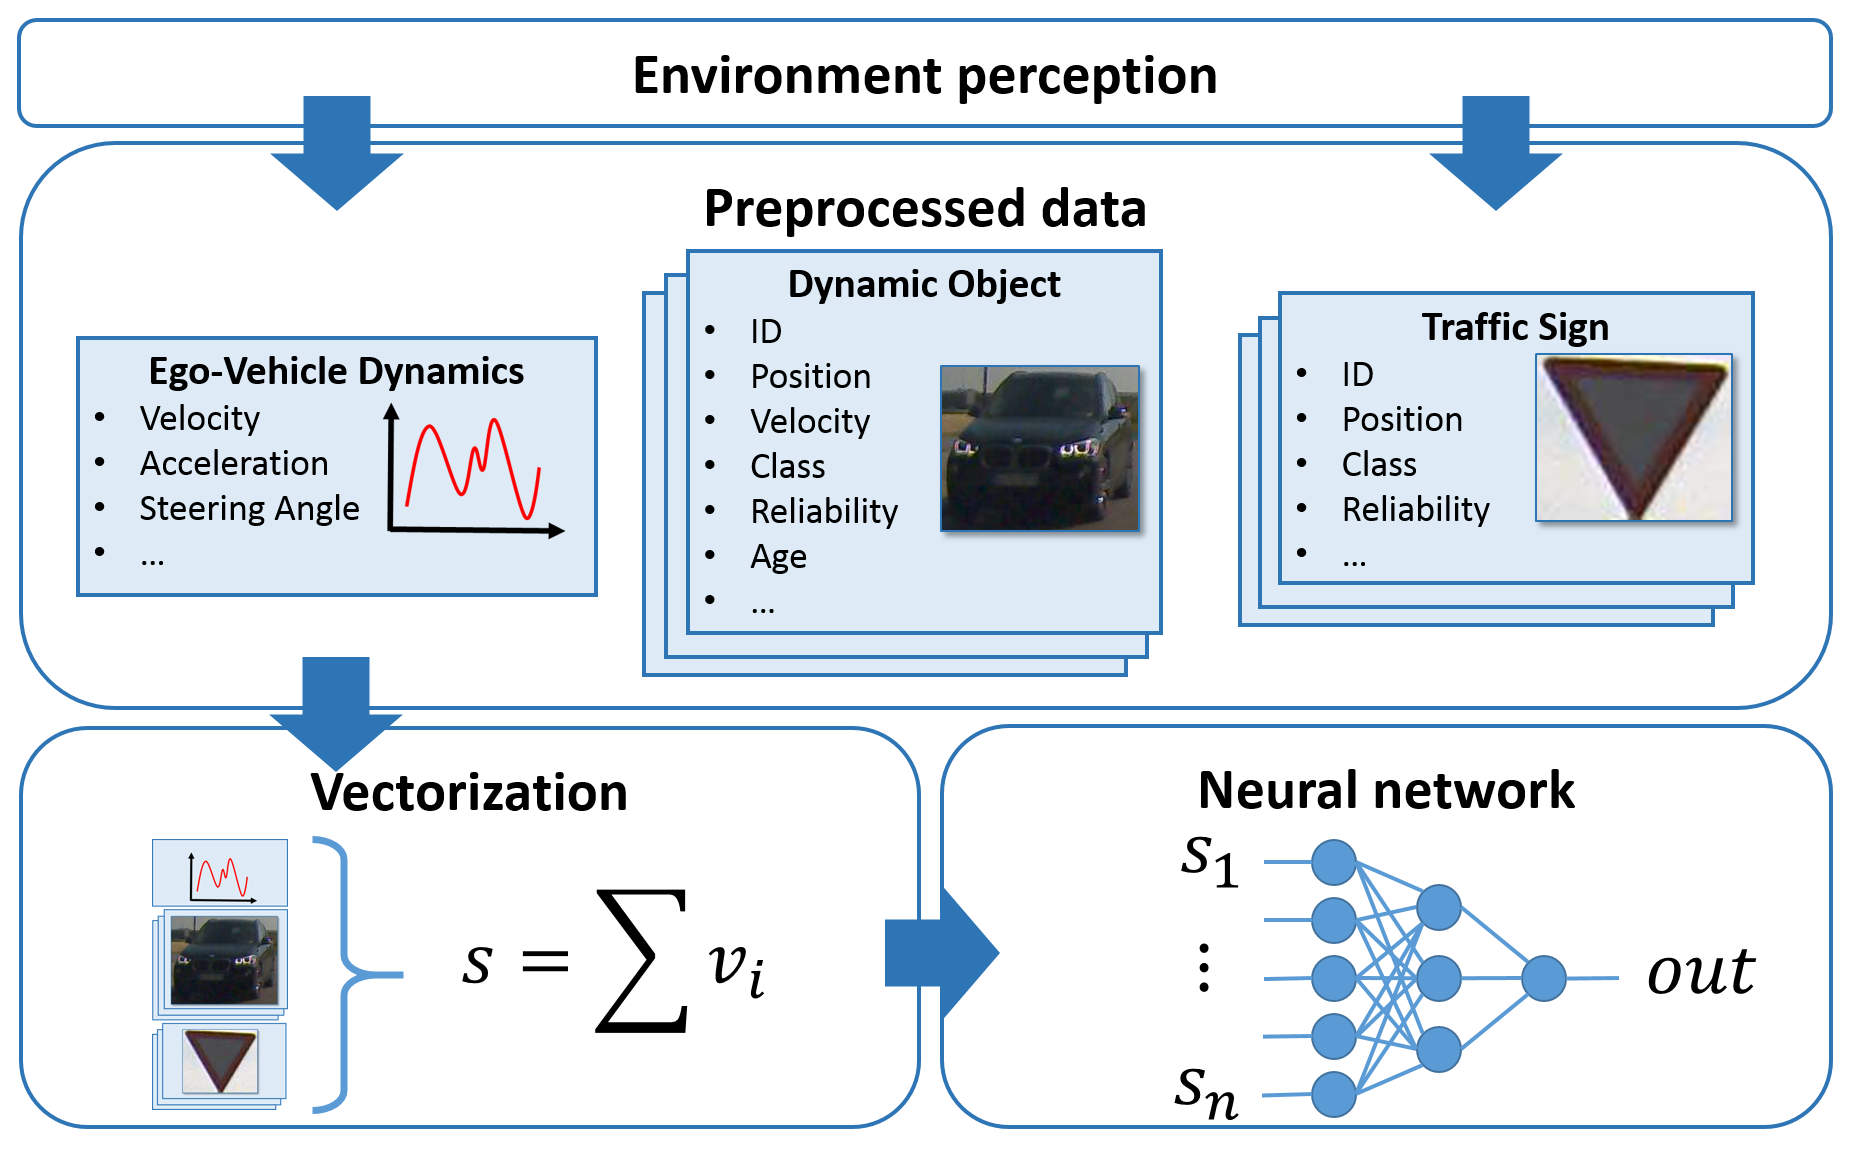
\includegraphics[height=3cm]{imgs/system_overview_horizontal.eps}
        }
    }
    \caption{Overview of the driving context classification system.
    ~\protect\subref{subfig:Example_scene} shows one example scene with objects of interest such as cars and traffic signs highlighted by colored bounding boxes.
~\protect\subref{subfig:system_overview_horizontal} illustrates the learning system's architecture and flow of information.}
    \label{fig:context_class_sys_arch}
\end{figure}

For the task of classifying the current driving context from measurements provided by the ego-vehicle's on-board sensors, we encapsulate three types of information in our vector-based scene representation, namely certain dynamics of the ego-vehicle, dynamic objects and traffic signs.
Information on all of these entities is provided as preprocessed object-lists as described in section~\ref{sec:data_and_preprocessing_context_classification}.
In subsequent sections, we describe the process of converting the input data into a vector representation for each of these categories of information.

\subsubsection{Ego-vehicle dynamics}
\label{subsubsec:ego-veh-dyn}

Regarding the dynamics of the ego-vehicle, we encapsulate the current velocity $\nu$, acceleration $(a_x, a_y)$ split in lateral and longitudinal direction with respect to the ego-vehicle's coordinate system  as well as the angle $\alpha_{steering}$ of the steering wheel, and the steering angle $\alpha_{axle}$ of the front axle.
Since all of these units are intangible concepts, we encode them by assigning a random vocabulary vector to each of them.
To represent the numerical value corresponding to each unit, we employ the simple scalar multiplication encoding introduced in section~\ref{ssubsec:scalar_multiplication_encoding}.
We illustrate this procedure for the current velocity of the ego-vehicle: let $ \mathbf{VELOCITY} = \left(v_0, \ldots, v_{D-1}\right)$ with $v_i \in \mathbb{R}$ for all $i=0, \ldots, D-1$ be the randomly chosen, normalized vocabulary vector representing the unit velocity, we encode the value $\nu$ of the ego-vehicle's velocity as $\nu \cdot \mathbf{VELOCITY}$.
Furthermore, we normalize all scalar values to the range $\left[-2,2\right]$ to keep the length of our vectors limited.
For vectorization of the two-dimensional acceleration values in longitudinal ($x$) and lateral ($y$) direction, we use the encoding based on sine and cosine functions with different spatial frequencies and offsets employing the function $\lambda$ introduced in Equation~\eqref{eq:cosin_2d_enc} in section~\ref{ssubsec:sine_cosine_based_representations}.
Hence, to obtain a vector representation of acceleration in longitudinal ($x$) and lateral ($y$) direction $(a_x, a_y)$, we use the encoding $\lambda\left(a_x, a_y\right)$, which leads to normalized, nonzero, similar vectors with information distributed over all elements.
To achieve the encoding of all dynamics of the ego-vehicle, we sum up the vectors representing the individual values, i.e.,
\begin{align}
\label{eq:ego_dynamics}
\mathbf{EGO}_{t} &= \nu \cdot \mathbf{VELOCITY} + \alpha_{steering} \cdot\mathbf{STEERING} \nonumber \\
             &+ \alpha_{axle} \cdot\mathbf{AXLE} + \lambda\left(a_x, a_y\right) \varoast \mathbf{ACCELERATION}
\end{align}
\subsubsection{Traffic participants}%
\label{ssubsec:traffic_participants_context_class}

The camera-based classification system is able to distinguish five different traffic participant categories, namely \emph{bicycle}, \emph{car}, \emph{motorcycle}, \emph{pedestrian} and \emph{truck}.
Furthermore, there are additional categories \emph{stationary} for stationary objects and \emph{unknown} for objects, where none of the aforementioned labels can be assigned to.
We generate vocabulary vectors for each traffic participant class.
In the simplest form of a vector representation, we could simply add the vocabulary vector once for each appearence of the corresponding object in the scene to the current representation vector. 
However, this representation just encodes that there are certain objects present somewhere in the current scene without any additional information.
To encode a more detailed representation of the current scene with additional information on each traffic participants position, we use the function $\lambda$ from Equation~\eqref{eq:cosin_2d_enc} again to map each dynamic object's position $(p_x, p_y)$ in longitudinal ($x$) and lateral ($y$) direction relative to the ego-vehicle's coordinate system to vector form $ \lambda(p_x, p_y)$.
Subsequently, we bind the resulting vector encoding the object's position to the vector representing the object's category.
However, positional information for each traffic participant might not be informative enough regarding the task of distinguishing between several driving contexts.
One quite unique feature of, for instance, highway driving is the fact that almost all other traffic participants drive in similar direction as the ego-vehicle.
Therefore, we create additional vocabulary vectors encoding the orientation of dynamic objects relative to the ego-vehicle for three discretized categories, namely $\mathbf{SAME}$, $\mathbf{OPPOSITE}$ and $\mathbf{OTHER}$, and  bind this orientation information to each dynamic object as we did for position information.
If we want to jointly attach those two pieces of information to one object, we need to generate two additional vocabulary vectors $\mathbf{POSITION}$ and $\mathbf{ORIENTATION }$ to impose structure.
For instance, a car detected at position $\left(p_x,p_y\right)$ with approximately the same orientation as the ego-vehicle would lead to the following vector representation
\begin{equation}
\label{eq:pos_orientation_context_class}
\mathbf{CAR} + \mathbf{CAR}\varoast\mathbf{POSITION}\varoast\lambda\left(p_x,p_y\right) + \mathbf{CAR}\varoast\mathbf{ORIENTATION}\varoast\mathbf{SAME}.
\end{equation}

Let all traffic participants in the current scene be given as $obj_{i}$ for $i=0, \ldots, n$, we get the vector encoding traffic participants as
\begin{align}
\label{eq:traffic_participants_context_class}
\mathbf{OBJ}_{t} &= \sum\limits_{i=0}^{n} \mathbf{TYPE}_{obj_i} + \mathbf{TYPE}_{obj_i} \varoast \mathbf{POSITION} \lambda\left(p_{x,i},p_{y,i}\right) \nonumber \\
                 &+ \mathbf{TYPE}_{obj_i}\varoast\mathbf{ORIENTATION}\varoast\mathbf{ORIENT}_{obj_i},
\end{align}
with $ \mathbf{TYPE}_{obj_i}$ denoting the vector representing the object's category and $ \mathbf{ORIENT}_{obj_i}$ denoting the vector representing the object's orientation.

\subsubsection{Traffic signs}%
\label{ssubsec:traffic_signs}

The ego-vehicle's camera-system is able to recognize a significant amount and variety of traffic signs.
We assign a vocabulary vector to each possible traffic sign label representing the corresponding traffic sign.
However, to generate a vector representation of all traffic signs relevant for the current driving context, it is not sufficient to simply add each currently visible sign to the current scene representation.
In contrast to traffic participants, there are many traffic signs, which are not only valid while being visible but stay relevant for the current driving context until withdrawn or overwritten by another sign.
For instance, if we observe a traffic sign indicating a speed limit of \SI[per-mode=symbol]{30}{\kilo\meter\per\hour}, that speed limit is valid and relevant until we encounter another traffic sign indicating a different speed limit.
Therefore, we implemented a simple form of memory for a certain subset of traffic signs relevant to the task of driving context classification even after disappearing from the field of view such as traffic signs indicating speed limits or traffic signs indicating the entrance or exit of a city or highway.
Due to the fact that the camera system is not immune to false detections, we implemented a decaying memory, to avoid relying too much on false detections and to allow the system to consider other cues as well.
We realized this decay by the function 
\begin{equation}
\label{eq:context_class_decay}
\sigma(t, \tilde{t}) = \gamma^{(\tilde{t} - t)},
\end{equation}
with a scaling factor $\gamma < 1$ and $ \tilde{t} > t$.
Furthermore, we include a simple logic to replace traffic signs in the representation if they are overwritten by more recently perceived ones.
For instance, recently observed traffic signs indicating a new speed limit overwrite previously seen speed limits and a sign indicating a city entrance withdraws a memorized highway sign.
Assuming we have encountered a particular sign $\mathbf{S}_{i}$ at time $t_{i}$, we achieve the vector encoding the traffic signs at time $t$ through
\begin{equation}
\label{eq:traffic_sign_context_class}
\mathbf{SIGNS}_{t} = \sum\limits_{i=0}^{n} \sigma(t, t_{i}) \cdot \mathbf{S}_{i} + \sum\limits_{j=0}^{m} \mathbf{\tilde{S}}_{j},
\end{equation}
for traffic signs $ \mathbf{S}_{i}$, which need to be memorized and traffic signs $ \mathbf{ \tilde{S}}_{i}$, which are only valid while they are visible.

\subsubsection{Putting it all together}%
\label{ssubsec:putting_it_all_together}

In the previous sections, we have presented the encoding process at time $t$ to generate vectors representing the dynamics of the ego-vehicle in $ \mathbf{EGO}_{t}$, the traffic participants or dynamic objects in the scene in $ \mathbf{OBJ}_{t}$ as well as the traffic signs either currently visible or memorized ones from previous observations in $ \mathbf{SIGNS}_{t}$.
To finally generate the vector representing the current scene, we simply sum up these individual pieces of information to
\begin{equation}
\label{eq:context_class_scene_vec}
\mathbf{SCENE}_{t} = \mathbf{EGO}_t + \mathbf{OBJ}_t + \mathbf{SIGNS}_t.
\end{equation}

We us these scene vectors as input for our classification model to classify the current driving context based on the current representation of the driving scene.

\subsection{Classification model}%
\label{subsec:classification_model}

In this section, we describe the model we use for classifying the driving context based on the vector representation of the current scene.
Our main model is a simple single-layer neural network implemented using the \ac{Nengo} \parencite{Bekolay2014} software suite, which is typically used to create large-scale neural models \parencite{Eliasmith2013}, but also allows the implementation of traditional feed-forward neural networks.
For the task of driving context classification, we use the \ac{LIF} neuron model and $N$ neurons in the hidden layer.
We employ supervised learning, i.e., we present the model with the vector representation as input and our manually generated driving context labels as output.
That is, we input the vectors encoding the current driving scene $\mathbf{v} = \left(v_{0}, \ldots, v_{D-1}\right)$ into $N$ neurons (encoding), and the output of the network (decoding) will be the classification $\mathbf{c}$ of the current driving context.
To encode the current scene vector in the activity $ \mathbf{a}_{i}$ of the $N$ neurons, we employ the principles of the \ac{NEF}:
\begin{equation}
  \mathbf{a}_{i} = \mathbf{G} \left(\sum_{j} \mathbf{e}_{i,j} v_j+\beta_i\right),
  \label{eq:context_class_encoding}
\end{equation}
where $ \mathbf{G}$ is the non-linearity of the neuron model and $\mathbf{e}_{i,j}$ and $\beta_i$ are randomly generated to produce a uniformly distributed range of maximum firing rates and intercepts.
To decode the classification of the current driving context from the neurons' activity $ \mathbf{a}_{i}$, we employ
\begin{equation}
    \mathbf{c} = \sum_{i=1}^{N} \mathbf{d}_{i}\mathbf{a}_i
  \label{eq:context_class_decoding}
\end{equation}
We leave $\mathbf{e}_{i,j}$ and $\beta_i$ at their randomly initialized values and use \ac{Nengo}'s default least-squares optimization to calculate the optimal decoder values $ \mathbf{d}_{i}$.

\section{Experiments}%
\label{sec:experiments_context_classificaiton}

In this section, we describe the experimental setup, models and metrics to analyze and evaluate our driving context classification model.
We present several reference models and human performance on the task of driving context classification in order to compare our model to.
Furthermore, we analyze the influence of variations in the underlying vector vocabularies on the classification accuracy.

\subsection{Performance baselines}%
\label{subsec:performance_baselines}

To get a better understanding of the quality the driving context classification model achieves based on our vector representation, we compare it to several other performance baselines.
In this section, we describe these reference models and the kind of data they use in comparison to the information encoded within our vector representation of the driving scene.
We use three baselines to compare our models performance to: human performance, a multi-layer neural network implemented using the Keras library \parencite{Chollet2015keras} using our vector representation as input data and a \ac{CNN} using raw images to classify the current driving context.

\subsubsection{Human performance}%
\label{ssubsec:human_performance}

\begin{figure}[t]
    \centering
    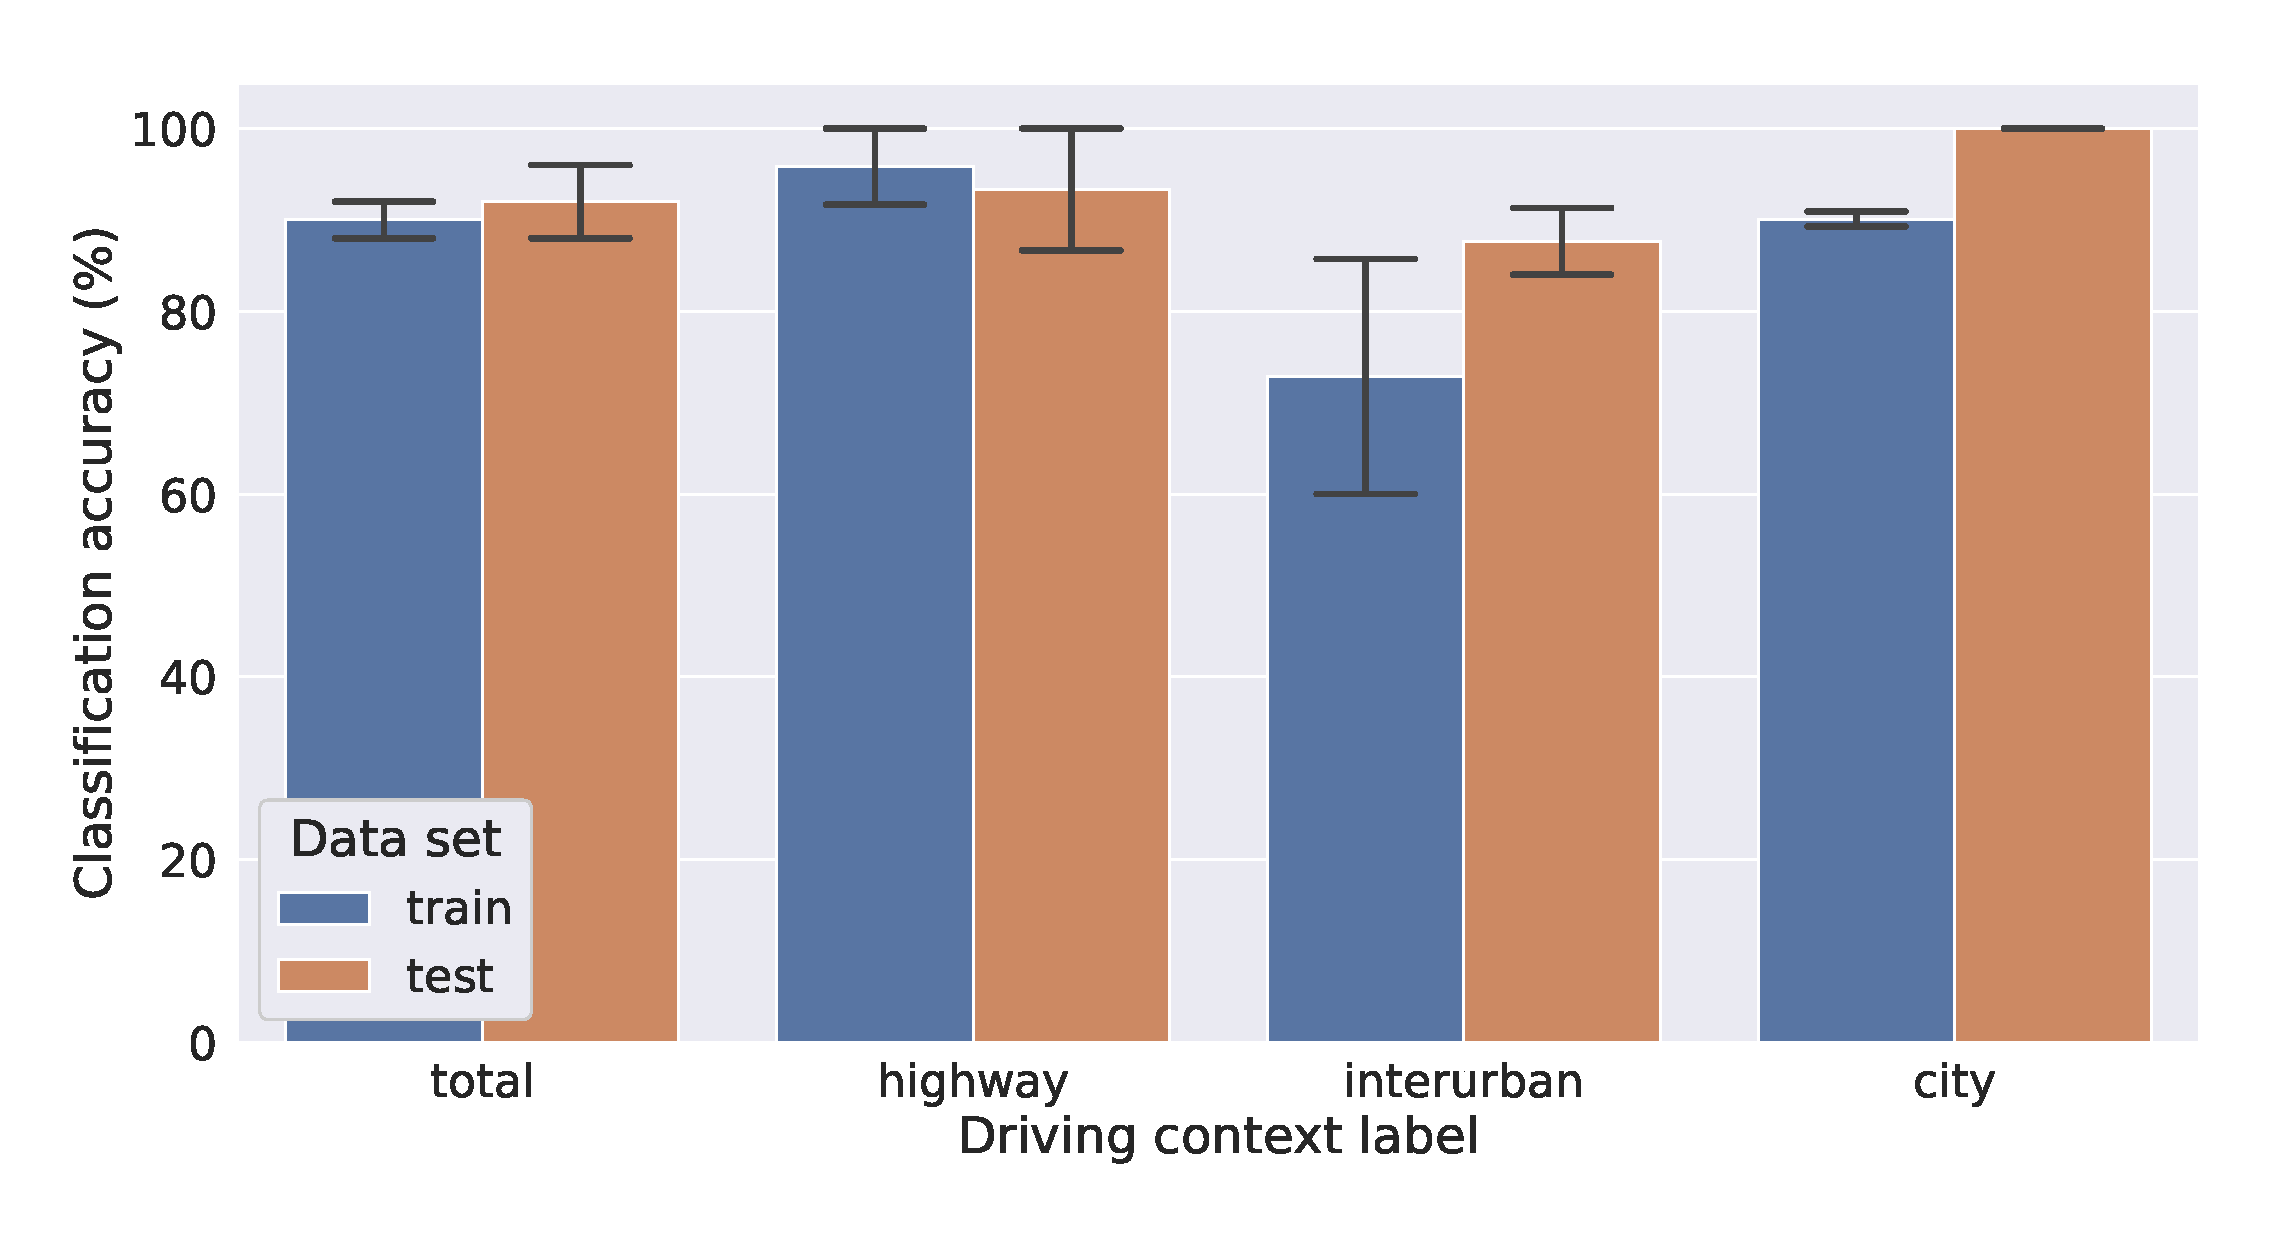
\includegraphics[width=1.0\linewidth]{imgs/context_class_human_train_test.eps}
    \caption{Classification performance of \num{2} human subjects on \num{50} examples selected randomly from each the training and test set.}
    \label{fig:context_class_human_train_test}
\end{figure}

One of the best and most competitive baselines for any learning model is the performance of humans in the task given to the learning system.
Hence, we also aim to compare our classification models' performance to that of human subjects on the same task.
However, we need to make sure that the data provided to the human subjects is as similar as possible to the information exposed to the learning system to make the results as comparable as possible.
The most intuitive way for human subjects to perceive and hence classify the current driving context would be through visual information, i.e., raw camera images.
However, the vector representation of the driving scene abstracts away most of the unnecessary visual features provided by the camera images and thus is very different information.
On the other hand, the raw numerical values of the vector representation are hard, if not impossible, to comprehend for human subjects.
Another intuitive way for humans to perceive information is language.
Therefore, we created human-readable versions of our input vectors in the form of written text by storing the label of the vocabulary vector followed by the encoded numerical value.
We presented a subset of \num{50} random samples for each data set to two human subjects asking for their classification guess.
To make this process as similar to the automated learning process pursued by the neural network, the human subjects had to classify samples from the training data set first.
After every sample, the subject was informed if the provided classification was correct or, in case of wrong classifications, which label would have been the correct answer.
In this way, we aim to provoke a steep learning curve for the human subjects before switching to the test set and replicate the learning process of the neural models as closely as possible.
Figure~\ref{fig:context_class_human_train_test} shows the performance for the two human subjects on both the training and test sets on the individual labels and their overall performance.
These results indicate that an overall classification performance of roughly \SI{92}{\percent} and at least \SI{80}{\percent} for the individual driving context labels are a reasonable baseline for the neural models to be compared to.

\subsubsection{Multi-layer neural network}%
\label{ssubsec:multi_layer_neural_network}

The first reference model to compare our spiking neuron based driving context classification model to is a more traditional feed-forward, multi-layer neural networks of rate neurons.
This model also uses our vector representation of the current driving scene as input and is trained in supervised fashion to classify the current driving context.
Here, we use a network consisting of several fully-connected hidden layers followed by a classification layer producing the models predictions.
This model is quite similar to our classification network with the most significant differences being the neuron models, i.e., \ac{ReLU} in contrast to the spiking \ac{LIF} neuron model in the \ac{Nengo} network version and the training procedure.
Both models employ supervised learning techniques and while the \ac{Nengo} model employs simple least squares optimization, the multi-layer Keras-model employs the classical backpropagation algorithm using gradient descent.

\subsubsection{Visual driving context classification using a \acs{CNN}}%
\label{ssubsec:visual_classification_using_cnn}

As mentioned earlier, a very intuitive way for us as human to classify the current driving context is by using visual information, i.e., raw images of the ego-vehicle's camera systems.
Many deep learning models, especially \acp{CNN}, are inspired by the structure of the human visual cortex and have achieved remarkable results on visual classification tasks.
Hence, we use a \ac{CNN} using the raw camera images as input data as our third and final reference model to compare our context classification network to.
We use a network architecture similar to the one employed in section~\ref{subsec:visual_vocabularies} to classify traffic signs based on visual input since this network architecture has been used successfully for classification tasks based on visual input.
The model is a multi-layer neural network with three convolutional layers each followed by a pooling layer with one additional fully connected layer and the final classification layer.
The network is trained using backpropagation and the classical gradient descent.

\subsection{Model training}%
\label{subsec:model_training}

In this section, we describe the process of training our context classification model as well as the aforementioned reference models.

\subsubsection{Nengo model training}%
\label{ssubsec:nengo_model_training}

As mentioned in section~\ref{subsec:classification_model}, we use \ac{Nengo}'s default least squares optimization to solve for the decoders $ \mathbf{d}_{i}$ in Equation~\eqref{eq:context_class_decoding}.
However, in order to generate the optimal decoders for the complete training set, we need to solve Equation~\eqref{eq:context_class_decoding} for all samples, i.e., each pair of scene vectors and true context labels  $ \left( \mathbf{v}_{j}, \mathbf{c}_j\right)$ for $j=0, \ldots, M$ in the training data set.
By default, this results in a matrix $A = \left( \mathbf{a}_{i,j}\right)$ for $i=0, \ldots, N$ and $j=0, \ldots, M$, with $N$ being the number of neurons in the population encoding the current scene vector and $M$ being the number of samples in the training set, which in our case is roughly \num{350000} samples.
Hence, in order to solve for the optimal decoders, \ac{Nengo} needs to generate a giant matrix $A$ of neural activities and store it in the system's memory in addition to the high-dimensional vectors in the training set.
That results in high memory requirements for the training process, which imposes restrictions on the computational hardware and could thus be prohibitive.
Therefore, we also implemented a variant of the training process, that calculates the matrix $A$ in blocks for subsets of the training samples of size $b < M$ and thus solves iteratively for the decoders $ \mathbf{d}_{i}$ for $i=0, \ldots, b-1$ and then for the next block $i=b, \ldots, 2b-1$ until we have calculated all decoders.
That slight adjustment is mathematically equivalent to the default least squares optimization process to solve for the decoders, but only consumes memory resources in the order of $ \mathcal{O}\left(N\cdot b\right)$ instead of $ \mathcal{O}\left(N \cdot M\right)$.
The only other difference is that we use regularization in the default least squares optimization method.
This is typically used to impose a certain amount of noise to make the learning population generalize better.
In our case however, we found that dropping this regularization leads to improved classification results (see section~\ref{subsec:evaluation_of_the_classification_performance})

\subsubsection{Multi-layer neural network training}%
\label{ssubsec:multi_layer_neural_network_training}

We implemented the multi-layer, feed-forward neural network as a reference model to compare our \ac{Nengo} classification model to using the Keras library \parencite{Chollet2015keras}.
We chose a simple feed-forward network architecture with two fully connected hidden layers consisting of \num{1500} and \num{500} \ac{ReLU} neurons respectively each followed by a dropout layer and a final classification layer.
In contrast to the \ac{Nengo} model, we use backpropagation and stochastic gradient descent to adjust the networks neural weights.

\subsubsection{\acs{CNN} training}%
\label{ssubsec:cnn_training}

The \ac{CNN} for image-based context classification is implemented using the Tensorflow library \parencite{Abadi2016}.
We use a similar architecture as the one used for traffic sign classification in section~\ref{subsec:visual_vocabularies} with \num{9} layers.
\begin{center}
    \begin{tabular}{c|c|c|c}
         Layer & Type & \# maps and neurons & kernel \\
		\hline
         0 & input & \num{3} maps of $256 \times 144$ neurons & \\ 
         1 & convolutional & \num{100} maps of $250 \times 138$ neurons & $7 \times 7$ \\
         2 & pooling & \num{100} maps of $125 \times 69$ neurons & $2 \times 2$ \\
         3 & convolutional & \num{150} maps of $123 \times 67$ neurons & $3 \times 3$ \\
         4 & pooling & \num{150} maps of $61 \times 33$ neurons & $2 \times 2$ \\
         5 & convolutional & \num{250} maps of $59 \times 31$ neurons & $3 \times 3$ \\
         6 & pooling & \num{250} maps of $29 \times 15$ neurons & $2 \times 2$ \\
         7 & fully connected & \num{300} neurons & $1 \times 1$ \\
         8 & fully connected & \num{3} neurons & $1 \times 1$ 
    \end{tabular}
    \captionof{table}{Layer by layer architecture of our reference \ac{CNN} for driving context classification.}
	\label{tab:context_class_cnn_arch}
\end{center}
This architecture is shown in table~\ref{tab:context_class_cnn_arch} consisting of three consecutive convolutional layers each followed by a max-pooling layer and two fully-connected layers for the final classification.
The network has two additional dropout layers, one after the convolutional layer part of the network dropping \SI{25}{\percent} of the neurons activity and one before the final classification layer dropping \SI{50}{\percent} activity.
The model is trained using backpropagation and the classical gradient descent algorithm.
We also employed early stopping since the model's validation loss did not significantly decrease after roughly \num{3500} epochs and the model's performance did not improve for longer training phases.

\subsection{Evaluation of the classification performance}%
\label{subsec:evaluation_of_the_classification_performance}

\begin{figure}[t]
    \centering
    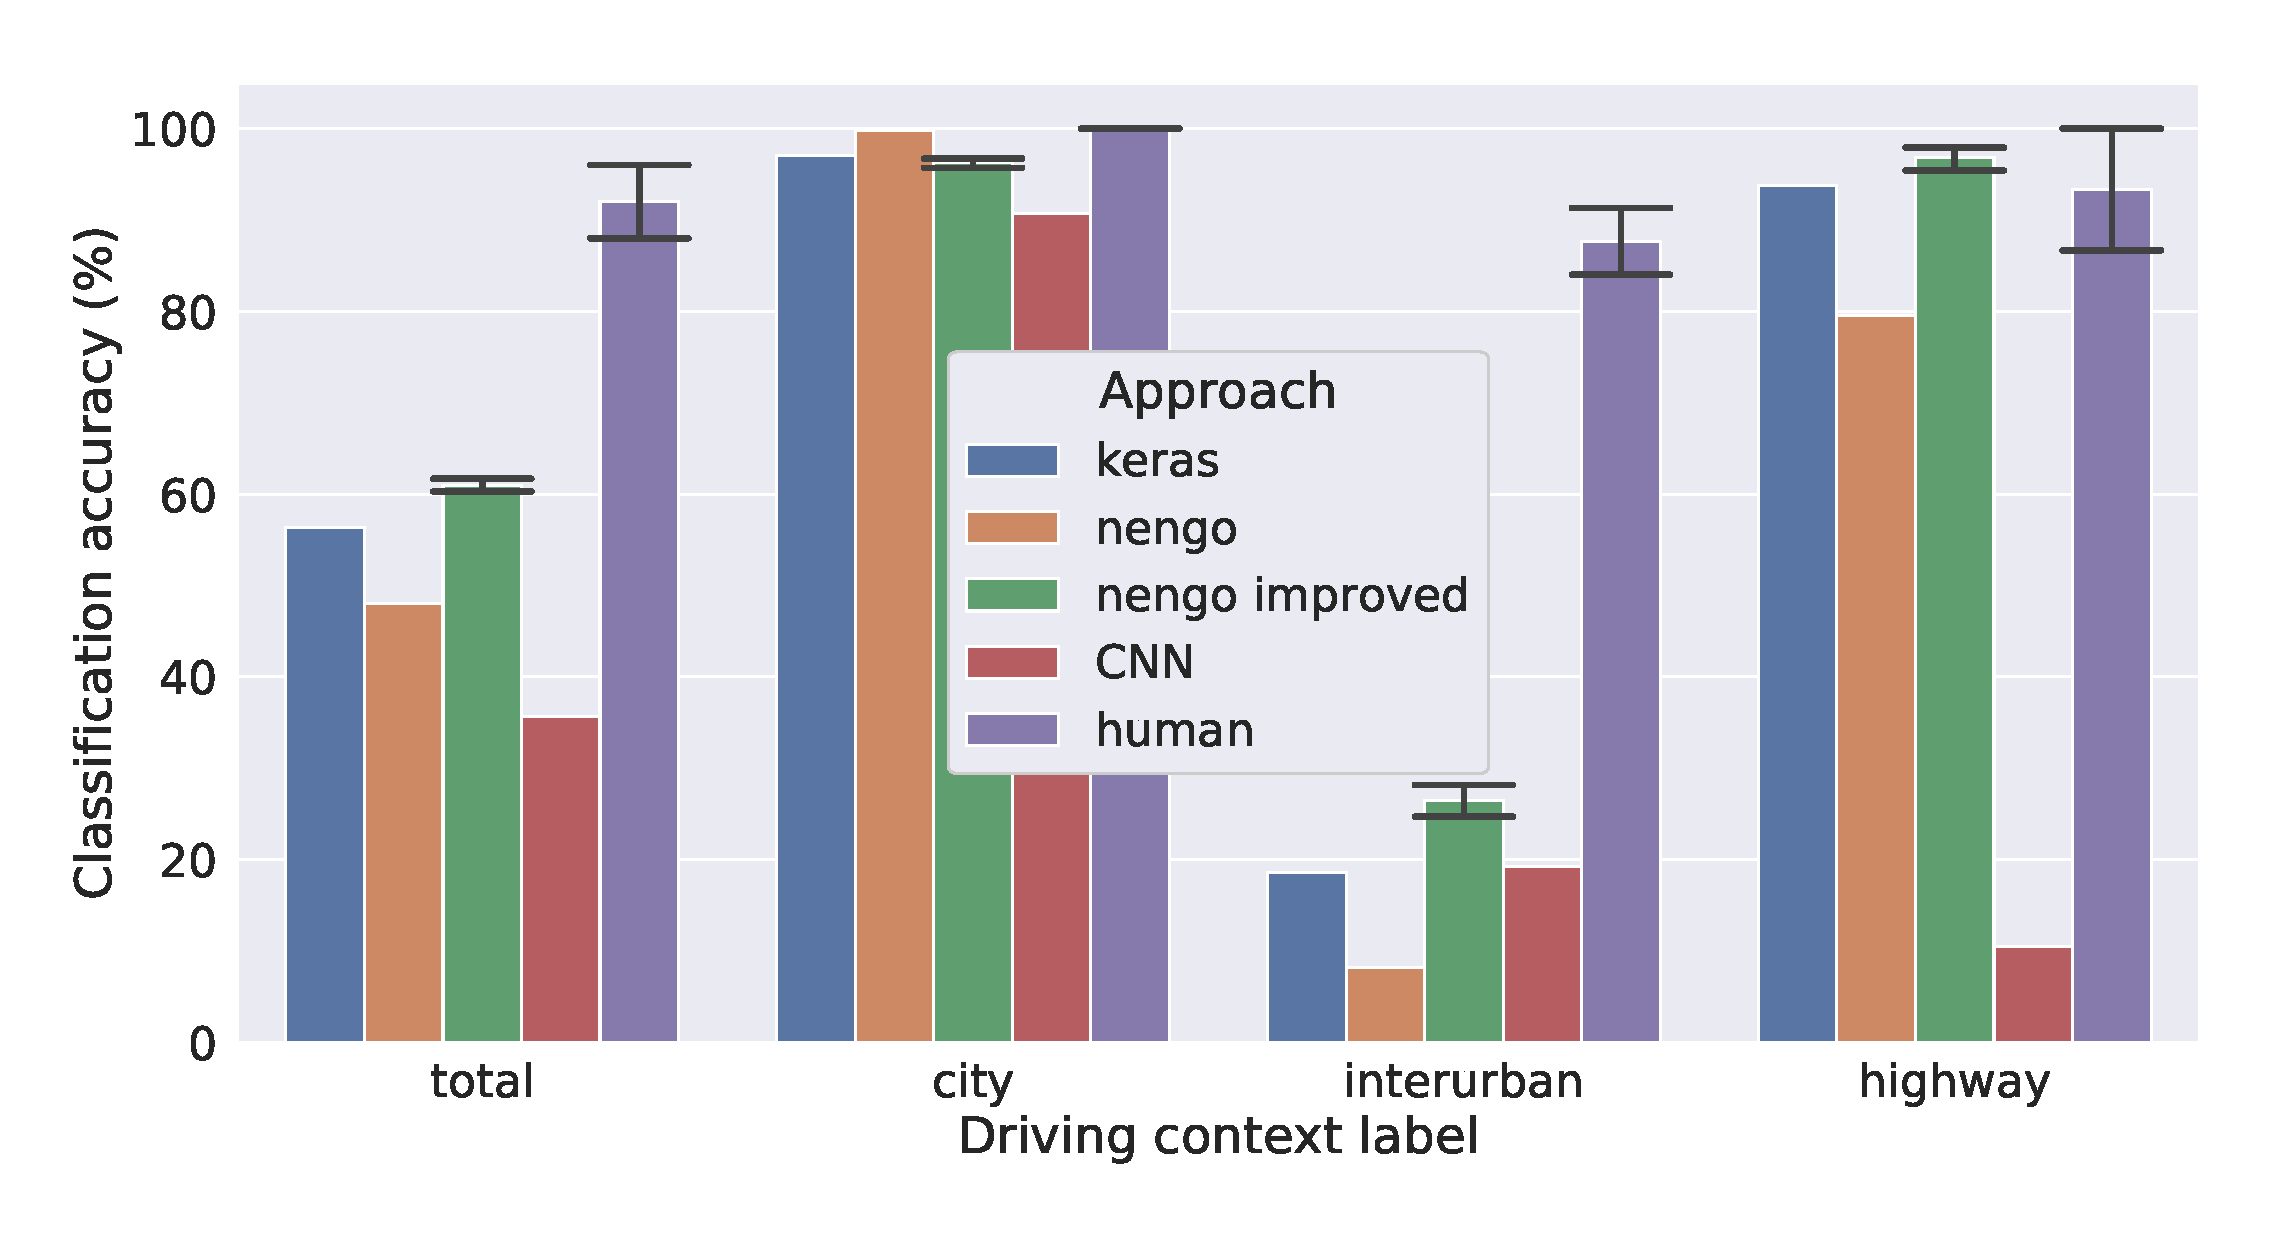
\includegraphics[width=1.\linewidth]{imgs/context_class_approaches.eps}
    \caption{Visualization of the performance of our driving context classification model and the comparison baselines for reference.}
    \label{fig:context_class_approaches}
\end{figure}

In this section, we analyze and evaluate the performance of our context classification model and compare it to the several baselines established in section~\ref{subsec:performance_baselines}.
Figure~\ref{fig:context_class_approaches} shows the classification performance for the \ac{Nengo} model, the multi-layer neural network implemented in Keras, the \ac{CNN} network based on raw camera images as well as the performance of our human subjects for reference.
In this section, we use random vocabularies of dimension \num{512} as basis for all the context classification models using our vector representation as input data.
The two variants of the \ac{Nengo} model referred to as \emph{nengo} and \emph{nengo improved} in Fig.~\ref{fig:context_class_approaches} differ in calculating the decoders on the complete set of training samples (\emph{nengo}) and on blocks of sample subsets (\emph{nengo improved}).
Furthermore, the \emph{nengo} variant uses regularization in the least squares optimization, namely \SI{10}{\percent} of the neurons activity, instead of no regularization in the \emph{nengo improved} model.
We observe that all automated learning models perform overall worse than the human performance baseline with the \ac{Nengo} model with improved and memory-efficient decoder calculation performs best with roughly \SI{62.6}{\percent} classification accuracy overall.
The second best classification performance achieves the Keras multi-layer neural neural network trained also on our vector representation performing just slightly worse than the best \ac{Nengo} model with a total classification accuracy of \SI{56.4}{\percent}.

\begin{figure}[t]
    \centering
    \subfloat[Complete test data set\label{subfig:context_class_prediction_vs_true_label}]{%
        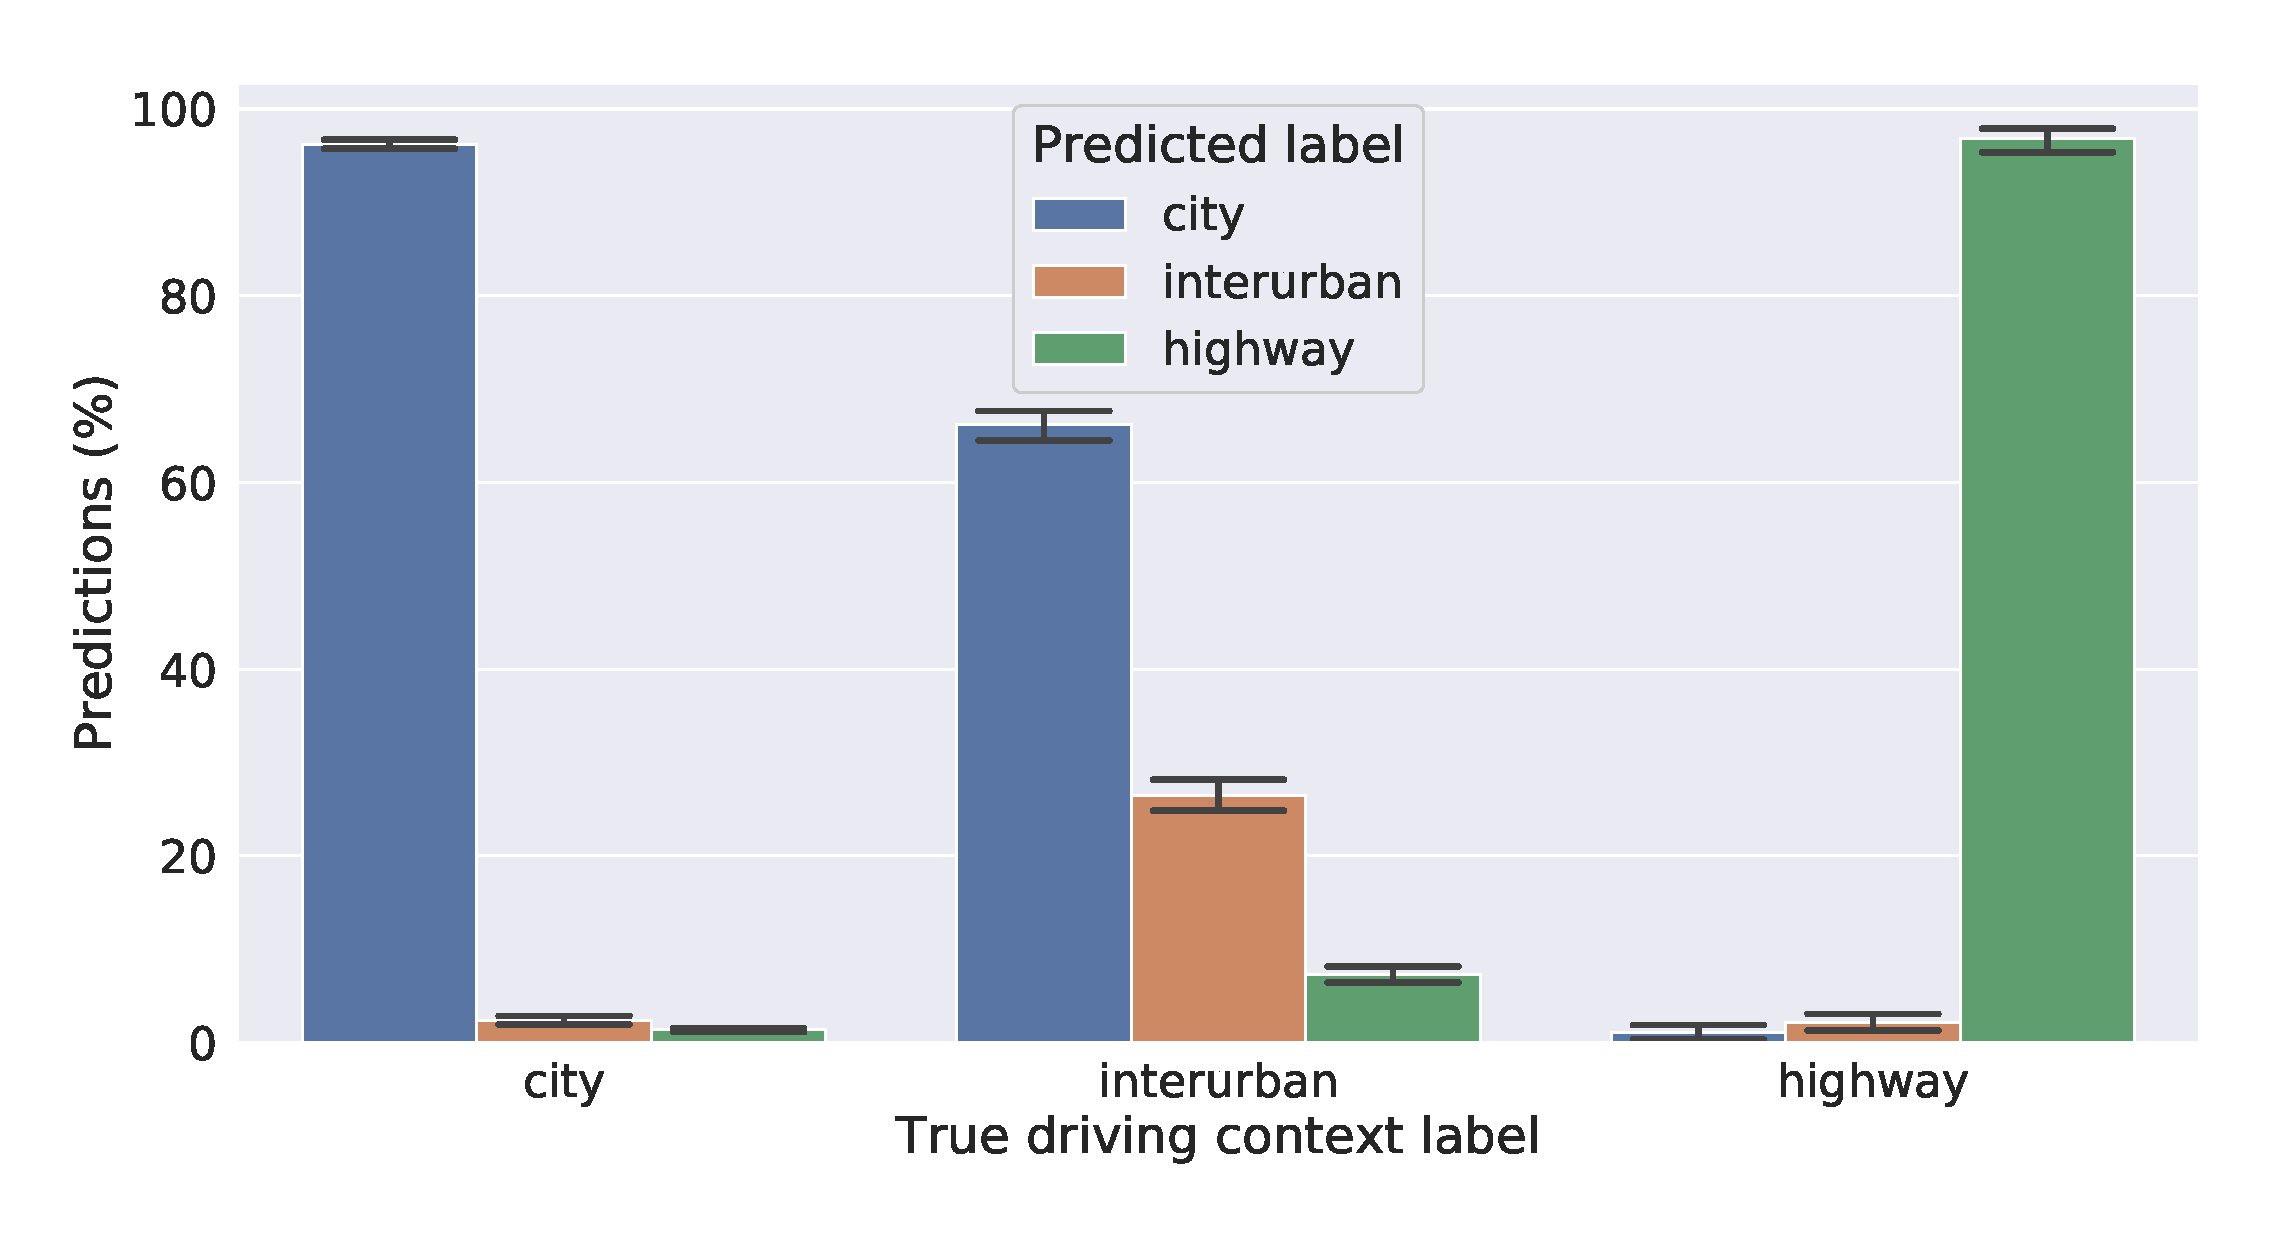
\includegraphics[width=0.5\linewidth]{imgs/context_class_prediction_vs_true_label.eps}
    }
    \subfloat[Subset of the test data set\label{subfig:context_class_prediction_vs_true_label_test_subset}]{%
        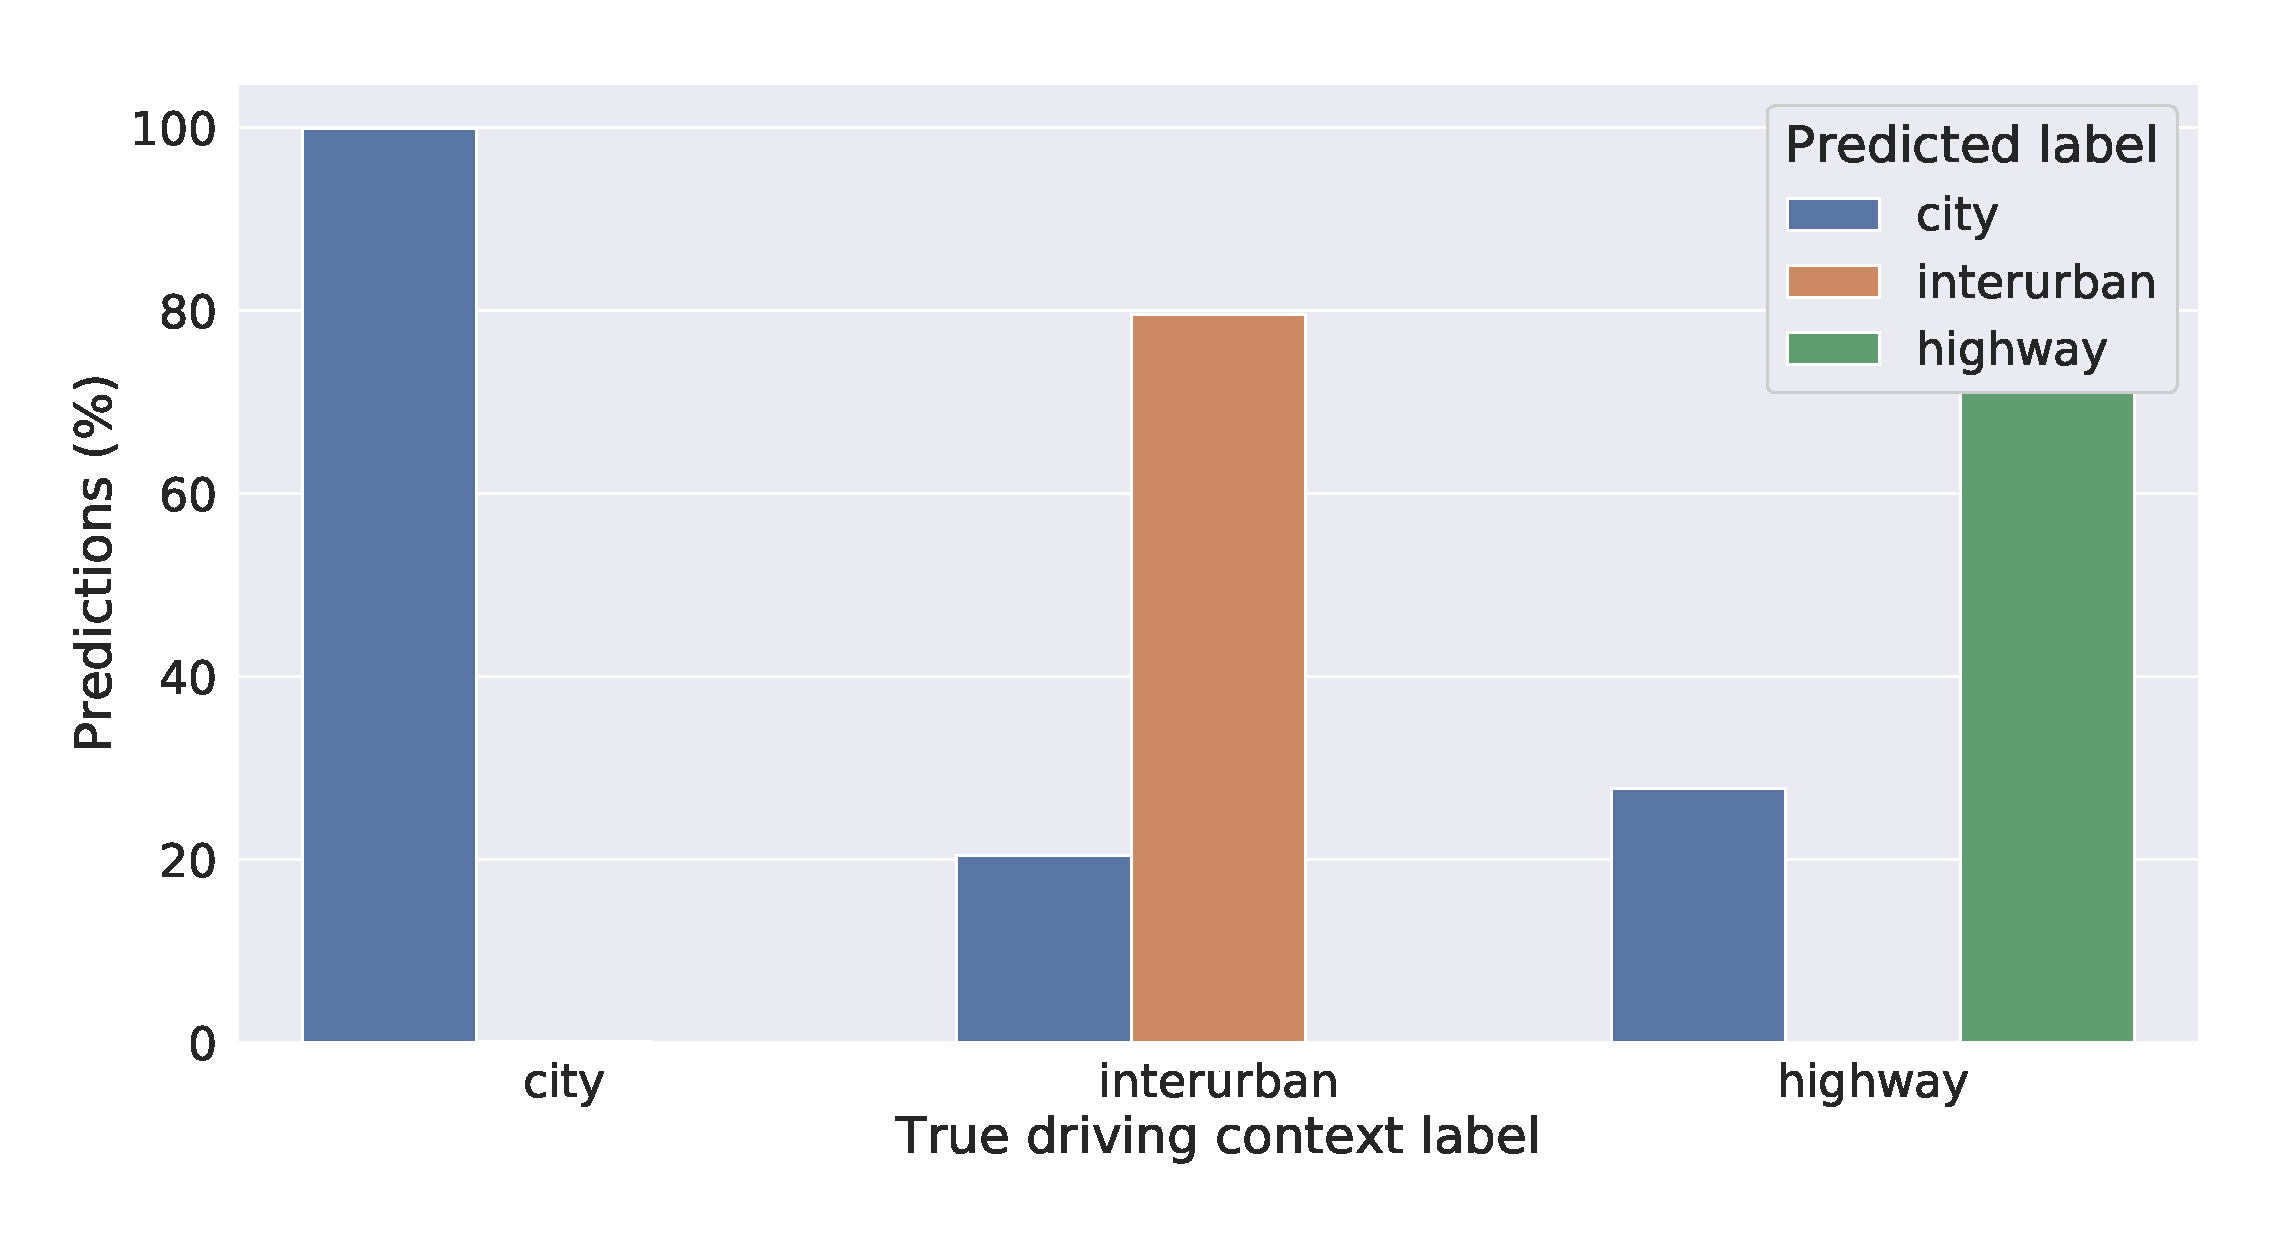
\includegraphics[width=0.5\linewidth]{imgs/context_class_prediction_vs_true_label_test_subset.eps}
    }\\
    \subfloat[Complete vs. test subset\label{subfig:context_class_test_subset}]{%
        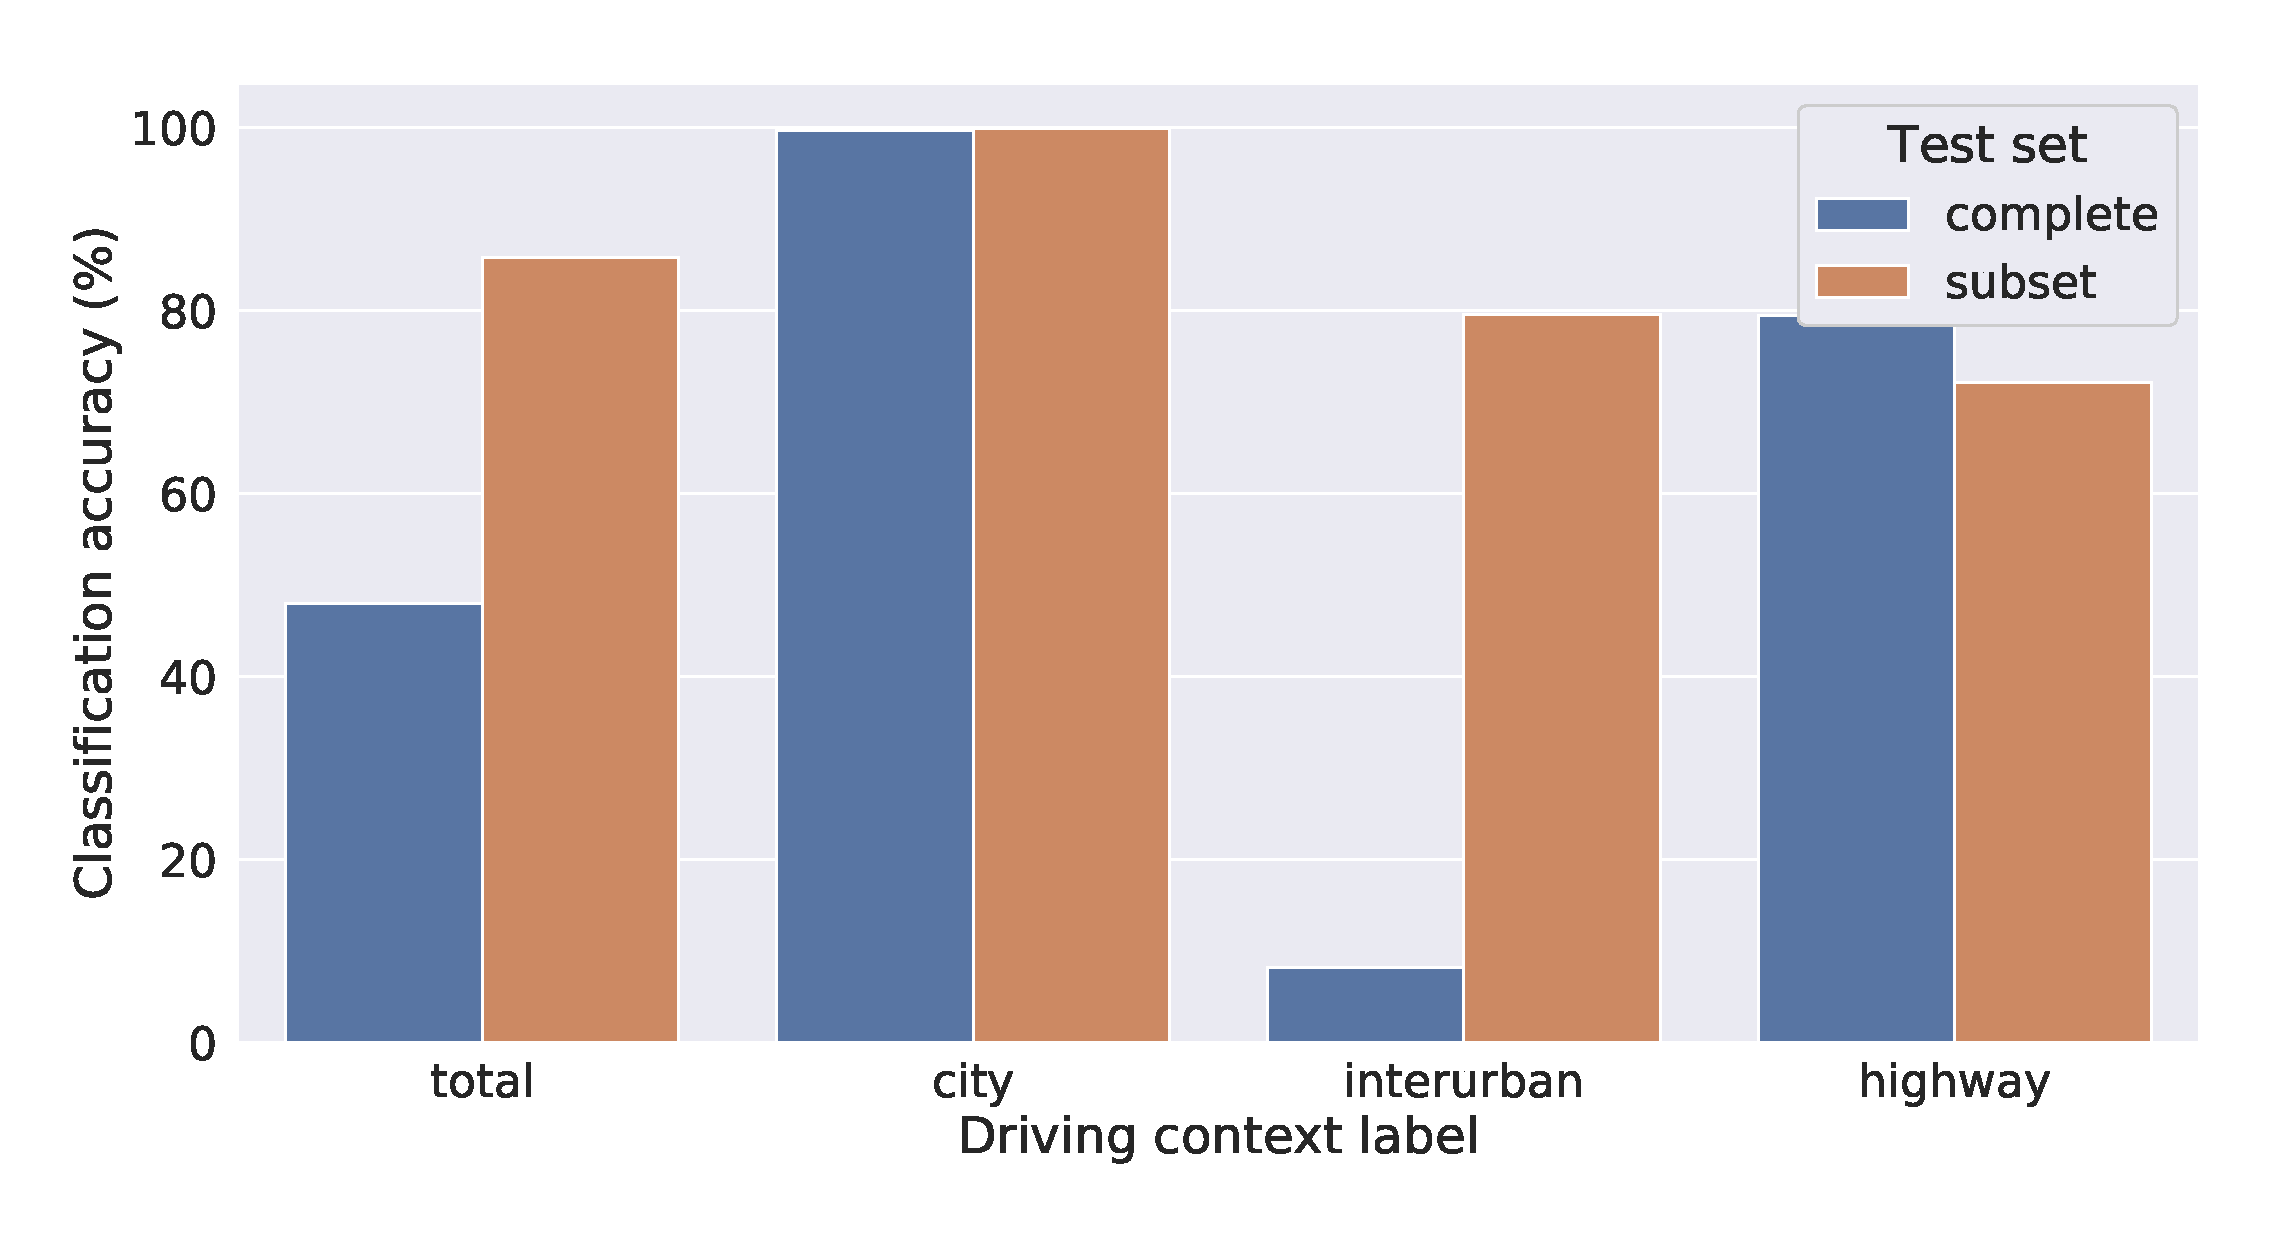
\includegraphics[width=1.\linewidth]{imgs/context_class_test_subset.eps}
    }
    \caption{Visualization of the driving context predictions made by the \ac{Nengo} model compared to the true labels. 
        Figure~\protect\subref{subfig:context_class_prediction_vs_true_label} shows the results for the complete test data set, while Fig.~\protect\subref{subfig:context_class_prediction_vs_true_label_test_subset} shows the model's predictions on the test subset compared to the true labels.
    Figure~\protect\subref{subfig:context_class_test_subset} shows the model's performance on the subset in comparison to the complete test set.
}
    \label{fig:context_class_test_subset}
\end{figure}
However, analyzing these results in more detail, we observe that the decreased overall classification performance for both, the \ac{Nengo} and Keras models is due to their poor classification performance on the \emph{interurban} context category achieving only \SI{27}{\percent} and \SI{18.6}{\percent} in comparison to the \SI{87}{\percent} classification accuracy achieved on average by the human subjects.
For the other context categories, \emph{city} and \emph{highway}, both models achieve competitive results comparable to the human classification performance baseline.
In order to further analyze this performance issue, we have a look at the composition of our data set.
The most critical problem is that our data is limited.
There are only \SI{18}{\minute} of test data available, which are recorded from just two test drives.
The first are \SI{4}{\minute} are continuous, mostly in the \emph{city} environment, with \SI{30}{\second} of \emph{interurban}, that are perfectly recognized.
The second part of the test set, again a continuous drive, contains, after starting in the \emph{city}, a long stretch of about \SI{8}{\minute} \emph{interurban} with heavy stop-and-go traffic at low speed.
The training set, however, does not contain data samples with driving situations comparable to that \emph{interurban} part in the test set.
Furthermore, the \emph{interurban} category is probably the most difficult to predict since there are \emph{interurban} samples that could be mistaken with either of the other two context classes depending on the situation.
Figure~\ref{subfig:context_class_prediction_vs_true_label} visualizes the amount of predictions of the \ac{Nengo} network for all the context classes compared to the true label of the data sample and supports these observations.
Although the majority of false classifications of the \emph{interurban} category is misclassified as \emph{city}, there is also a significant amount of samples mistaken for \emph{highway}.
On the other hand, \emph{interurban} is the category with the least amount of samples in the training data set as only \SI{18.9}{\percent} of the training samples belong to the \emph{interurban} class.
Thus, we assume that a more balanced and/or larger data set could be essential to tackle this issue.

Hence, we evaluated our classification model on a subset of the test set simply removing that \emph{interurban} part both model variants struggle to predict.
Figure~\ref{subfig:context_class_test_subset} shows the results of the original \ac{Nengo} classification network (i.e., trained without the memory-efficiency and regularization improvements) on the complete test set as well as on the subset, while Fig.~\ref{subfig:context_class_prediction_vs_true_label_test_subset} shows a similar evaluation for the subset of the training set as Fig.~\ref{subfig:context_class_prediction_vs_true_label} for the complete test set.
We observe that, even for this non-optimized model variant, the classification accuracy of the \emph{interurban} category significantly increases from \SI{8.1}{\percent} to \SI{79.5}{\percent} when switching from the complete test set to the smaller subset.
Thus, we consider this a strong hint that a more balanced and larger training data set will be able to improve the poor classification performance on the \emph{interurban} driving context category and therefore the overall accuracy of the model.

\begin{figure}[t]
    \centering
    \subfloat[\label{subfig:context_class_interurban_img} Interurban]{%
        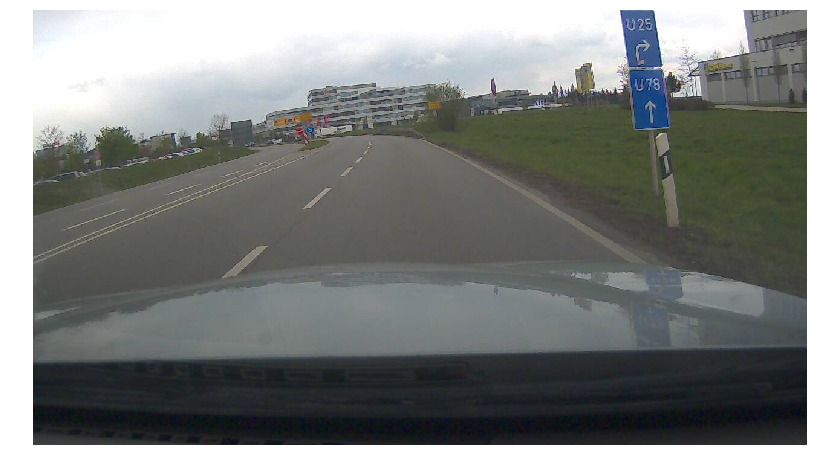
\includegraphics[width=0.5\linewidth]{imgs/context_class_interurban_img.png}
    }
    \subfloat[\label{subfig:context_class_city_img} City]{%
        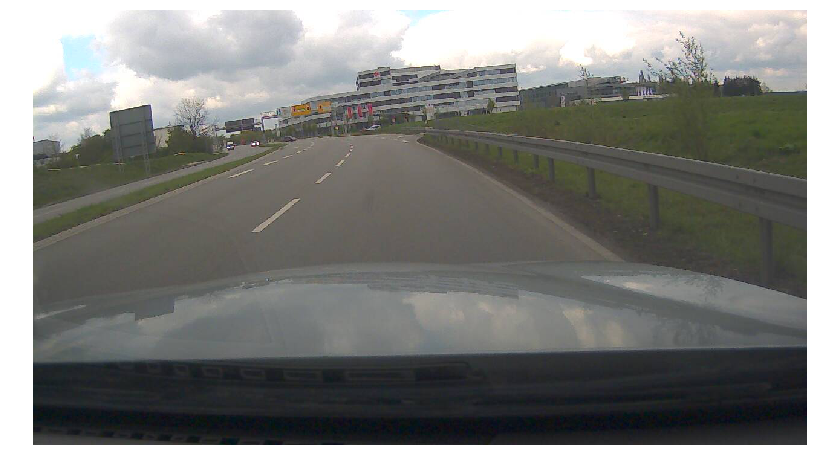
\includegraphics[width=0.5\linewidth]{imgs/context_class_city_img.png}
    }
    \caption{Examples of similar looking images in the test set with different driving context labels. }
    \label{fig:context_class_similar_image_examples}
\end{figure}

Revisiting Fig.~\ref{fig:context_class_approaches}, the \ac{CNN} classification model based on the raw camera images performing poorly in comparison to the other models achieving only \SI{35.7}{\percent} overall classification accuracy is sort of an exception.
While the model achieves \SI{90.7}{\percent} classification accuracy on the \emph{city} context label, its performance deteriorates down to \SI{19.2}{\percent} and \SI{10.5}{\percent} for the \emph{interurban} and \emph{highway} labels respectively.
This is even the best classification performance we were able to achieve with this model: when training the network for a larger amount of epochs, which, in theory, should improve the model's performance, its performance deteriorates even further.
Instead of generalizing better, the model tends to overfit and just learns to simply assign the same context label to all samples.
We assume, that there are too few and too similar images in the training data set for the model to sufficiently generalize beyond these samples.
For instance, Fig.~\ref{fig:context_class_similar_image_examples} shows two raw images from the training data set with rather similar visual features but with different labels.
Figure~\ref{subfig:context_class_interurban_img} shows a training sample of the \emph{interurban} category while Fig.~\ref{subfig:context_class_city_img} shows a \emph{city} sample.
Hence, we conclude that for the particular task of driving context classification performed on a rather small data set, it is beneficial to omit unnecessary visual features and complexity and instead use our abstract vector representation of the scene as input for an automated learning system.

\subsection{The influence of varying vocabularies}%
\label{subsec:the_influence_of_varying_vocabularies}

In section~\ref{sec:preprocessing_stage_generating_a_vocabulary}, we have already seen several ways to generate a vocabulary of atomic vectors for scene representation in automotive context.
For the evaluation in section~\ref{subsec:evaluation_of_the_classification_performance}, we focused solely on randomly generated vector vocabularies for the sake of simplicity.
Here, we are interested how varying vector vocabularies encapsulating a similarity structure of the encoded entities influence the performance on the task of driving context classification.

\subsubsection{Random vocabulary baseline}%
\label{ssubsec:random_vocabulary_baseline}

\begin{figure}[t]
    \centering
    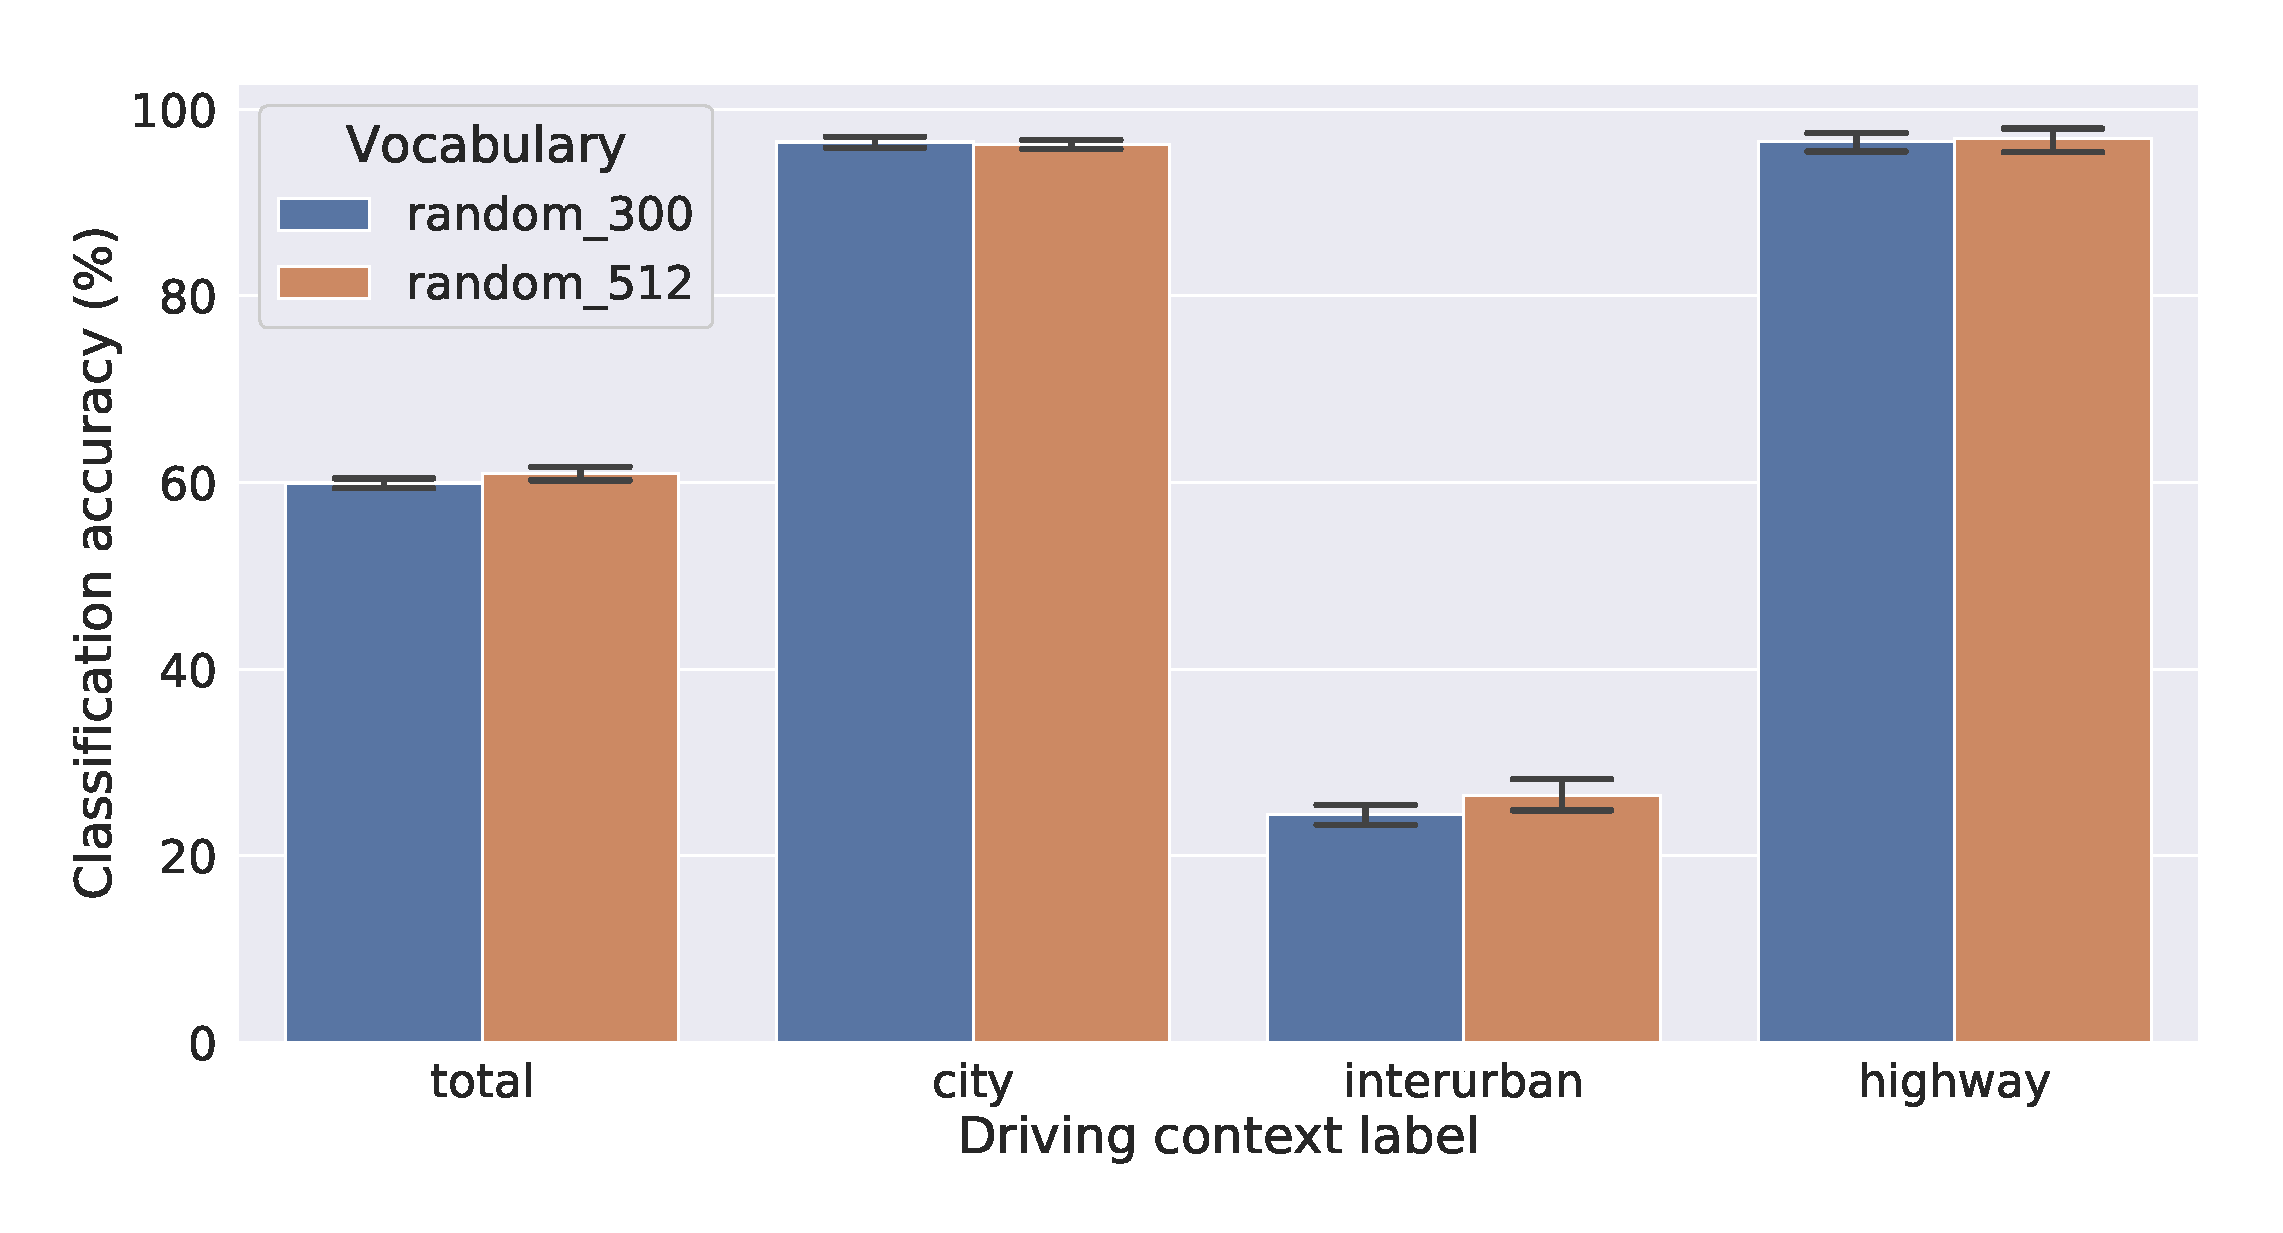
\includegraphics[width=1.\linewidth]{imgs/context_class_random_512_vs_random_300_dim_vocab.eps}
    \caption{Comparison of the driving context classification model for \num{300}-dimensional and \num{512}-dimensional vectors.}
    \label{fig:context_class_random_512_vs_random_300_dim_vocab}
\end{figure}

The evaluation in section~\ref{subsec:evaluation_of_the_classification_performance} was conducted on randomly generated vocabularies containing \num{512} dimensional vectors.
However, the structured vocabularies generated in section~\ref{sec:preprocessing_stage_generating_a_vocabulary} consist of \num{300} dimensional vectors.
Therefore, we first analyze how the reduced dimensionality of the underlying vector vocabulary influences the classification performance of our model.
Figure~\ref{fig:context_class_random_512_vs_random_300_dim_vocab} illustrates the performance of our \ac{Nengo} driving context classification model for \num{10} different randomly chosen vocabularies containing \num{300}-dimensional and \num{512}-dimensional atomic vectors.
Although we observe a slight deterioration of the classification accuracy when reducing the dimension of the vocabulary vectors, the difference is not statistically significant.
Hence, we use the classification performance on the \num{300}-dimensional random vector vocabularies as baseline for comparison for models built upon structured vocabularies encoding different types of similarity.

\subsubsection{Structured vocabularies}%
\label{ssubsec:structured_vocabularies}

\begin{figure}[t]
    \centering
    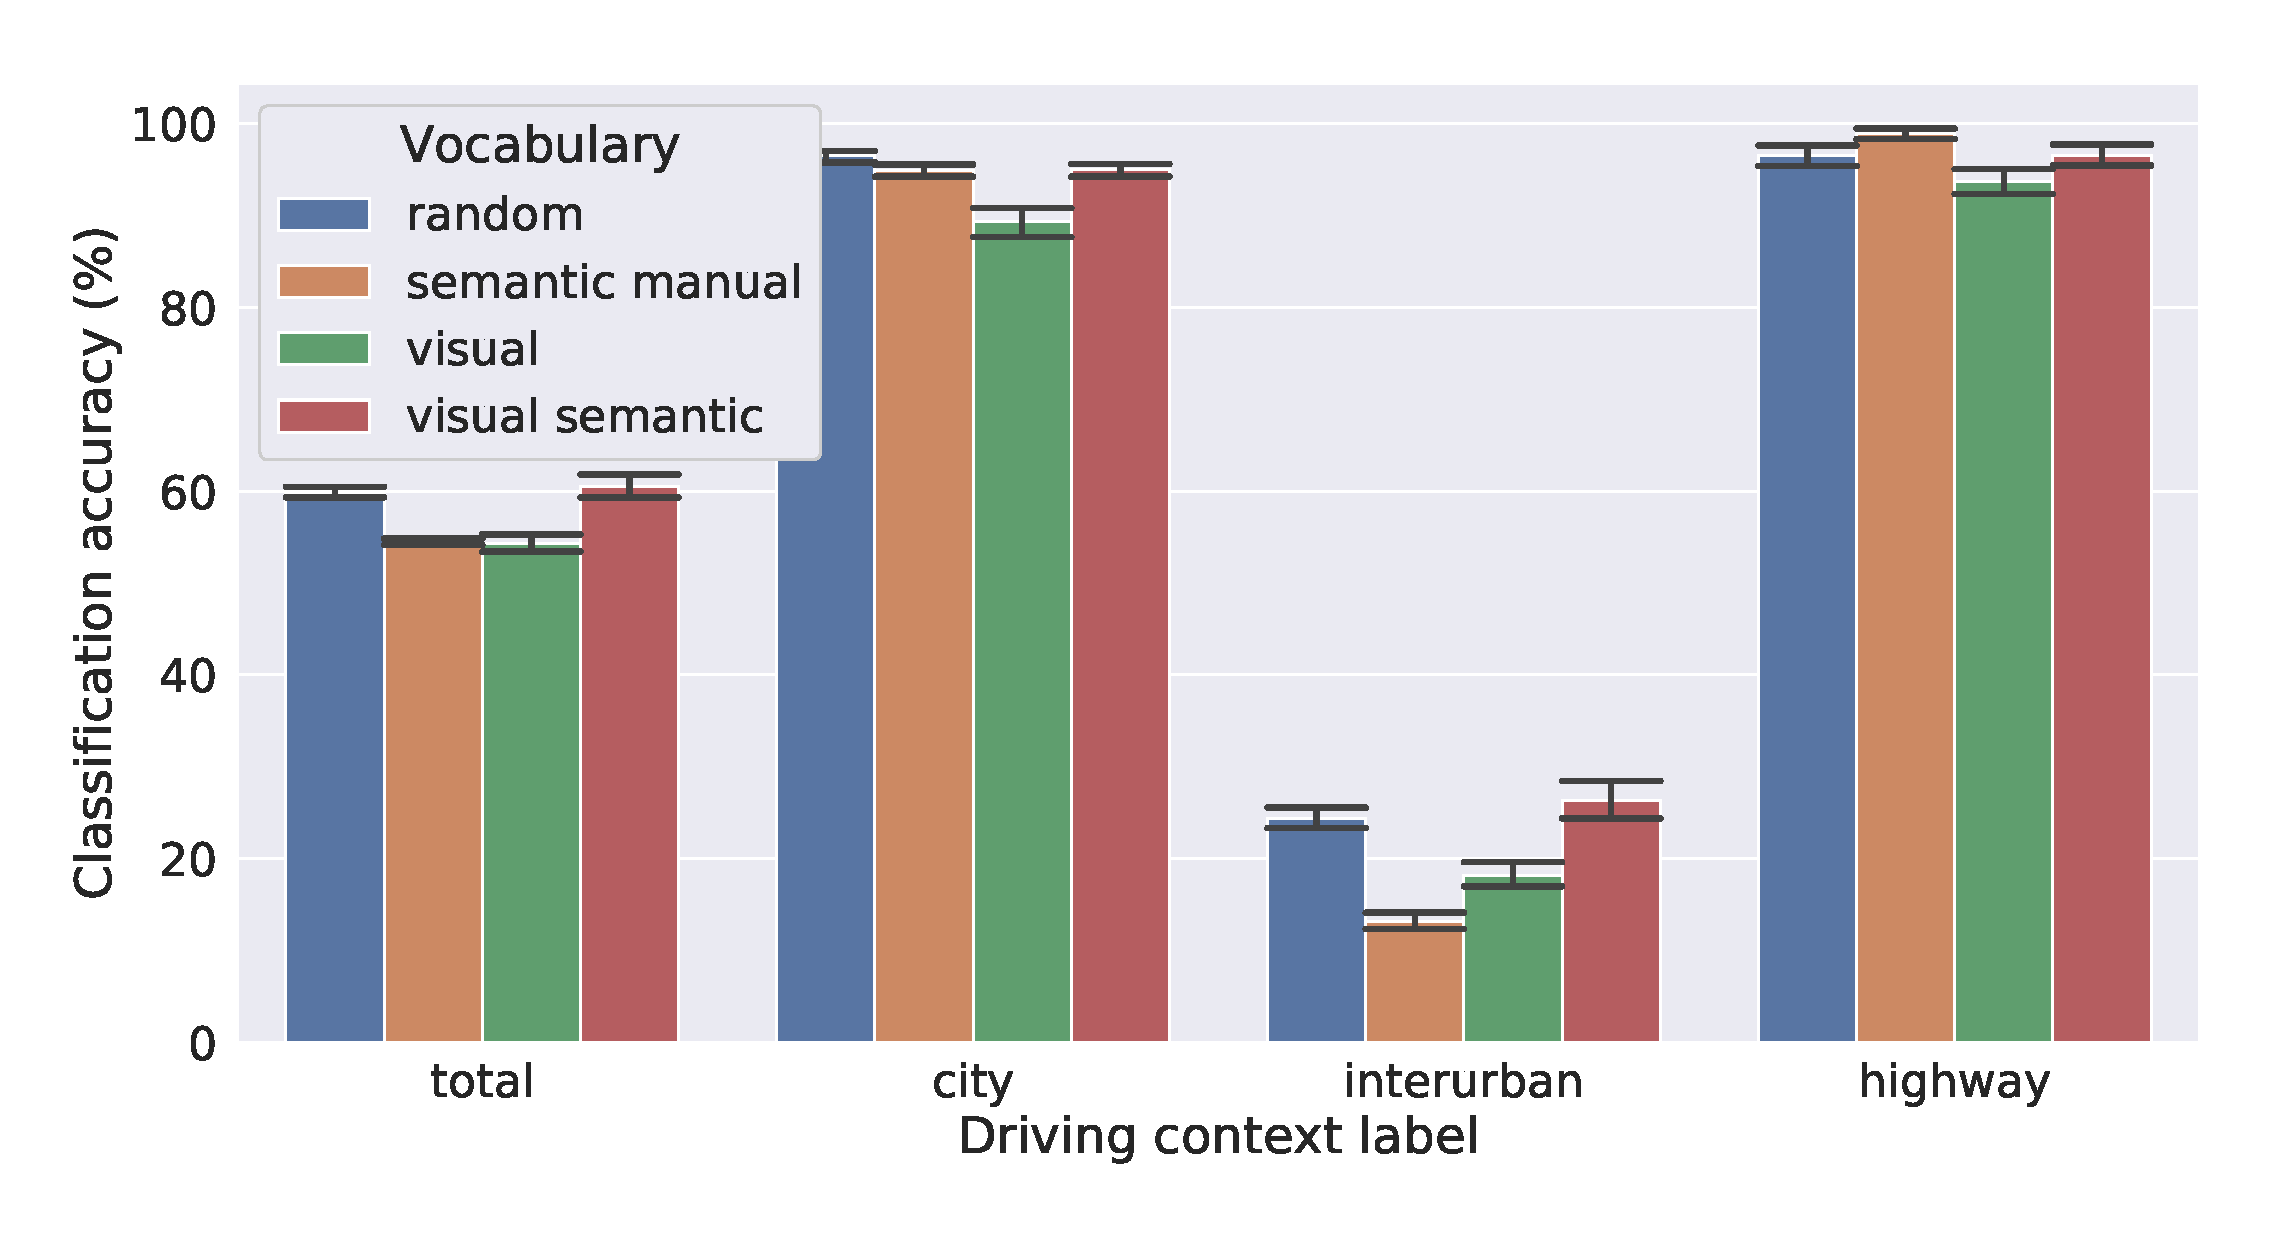
\includegraphics[width=1.\linewidth]{imgs/context_class_vocabularies_tp_and_ts.eps}
    \caption{Visualization of the \ac{Nengo} model's classification performance for several structured vocabularies compared to the baseline performance on randomly generated vocabularies.}
    \label{fig:context_class_vocabularies_tp_and_ts}
\end{figure}

In this section, we analyze the impact of encapsulating a similarity structure within the vocabulary of atomic vectors used to generate the scene representation vectors.
We hypothesize, that encapsulating a similarity structure within the vocabulary of atomic vectors is beneficial in terms of performance for our driving context classification model based on the scene representation built upon these vocabularies.
We use the different vocabularies presented in section~\ref{sec:preprocessing_stage_generating_a_vocabulary} to impose different similarity structures to the vocabulary, namely a manually generated semantic vocabulary (see section~\ref{subsec:semantic_vocabularies}), a learned visual vocabulary (see section~\ref{subsec:visual_vocabularies}) as well as a fused visual-semantic vocabulary combining the visual and semantic similarity structures in one vocabulary (see section
~\ref{subsec:visual_semantic_vocabularies}).
However, the aforementioned structured vocabularies do not contain all entities encoded in the random vocabularies.
For instance, the \ac{GTSRB} data set, which was used to generate the visual vocabulary for traffic signs, contains only \num{42} traffic sign classes, which covers only $\frac{1}{6}$ of the traffic signs the ego-vehicle's camera system is able to detect.
This allows us to encode the structure of, for example, speed limit signs as well as priority signs, which occur in both, our structured vocabulary and the driving data.
On the other hand, we do not encode the traffic sign indicating a speed limit of \SI[per-mode=symbol]{130}{\kilo\meter\per\hour} (as it is not contained in the \ac{GTSRB} data set), nor the signs indicating a highway entrance, which occur in the driving data and have a significant impact on the driving context classification.
Hence, we adapt the baseline random vocabularies by replacing the vectors with their counterpart within the structured vocabulary if such a vector exists and otherwise leave it unchanged.
Thus, we are only able to encode the desired structure for the subset of entities encoded in the vocabularies.

Figure~\ref{fig:context_class_vocabularies_tp_and_ts} illustrates the classification performance of our driving context classification model for the three different approaches to generate structured vocabularies as well as the random vocabularies as baseline. 
It shows the performance over \num{10} randomly generated vocabularies used as baseline as well as the starting point for structured vocabularies.
We observe the general trend that both, the manually generated semantic vocabulary as well as the vocabulary encapsulating visual similarity deteriorate the model's classification accuracy.
While the semantic similarity is able to slightly improve the classification accuracy at least for the \emph{highway} category, the classification performance for the model using the visual vocabulary decreases significantly for all context categories.
On the other hand, the vectors combining visual and semantic similarity in one vocabulary are able to slightly improve the model's accuracy over the random vocabularies.
Although the model's performance based on this visual-semantic vocabulary decreases slightly for the \emph{city} category, its performance on the \emph{highway} class is comparable and, on average, slightly improved for the \emph{interurban} context category.
For some individual vocabularies, the additional structure significantly improves results.
In the most extreme case, we observe an unchanged \SI{96}{\percent} prediction accuracy of \emph{city}, while \emph{interurban} increases from \SI{23}{\percent} to \SI{30}{\percent} and \emph{highway} from \SI{95}{\percent} to \SI{99}{\percent}. 
On the other hand, there are also vocabularies without substantial changes and, in some cases, even decreased classification performance.
For the most pronounced example, accuracy decreases in all three classes with a deterioration of \num{1} and \num{2} percentage points for \emph{city} and \emph{highway} respectively and even \num{5} percentage points for the \emph{interurban} category.

In conclusion, encapsulating visual semantic structure produces a measurable effect on the model's classification performance for several vocabularies and improves average results compared to the vocabularies encoding individual parts of the structure (i.e., only visual or semantic).
We observe a difference in classification accuracy of up to \SI{7}{\percent}.
However, the impact varies depending on the underlying original vocabulary: for some vocabularies, accuracy decreases over all classes, in others it increases.
On the other hand, since this average is only based on \num{10} vocabularies (due to computational limitations), this visual-semantic structure does not perform significantly better than the baseline vocabulary.
Furthermore, there is no  clear pattern observable such as an increase in accuracy especially for vocabularies that underperformed without additional structure, or a decrease for vocabularies that performed well using the original randomly generated vectors.

\section{Summary}%
\label{sec:summary_context_classification}

In this chapter, we have presented a novel approach to a data-driven driving context classification model based on our vector representation of driving scenes.
We proposed a vector representation of the current driving situation encapsulating a mixture of symbol-like information such as traffic signs or the type of traffic participants as well as numerical information such as position or velocity of dynamic objects.
We showed that our learning model using \acp{SNN} in the \ac{Nengo} framework outperformed the feed-forward reference neural network implemented in Keras as well as a \ac{CNN} based on raw camera images.
We assume that we successfully abstracted away unnecessary and too complex visual features from the representation for being able to learn driving context classification from a rather small vocabulary.
The \ac{CNN} would most likely require a much larger training data set containing a great variety of different examples of driving context examples under several conditions (e.g., daylight and night, heavy or flowing traffic etc.).
All data-driven models presented here performed worse than the baseline of human level performance, but mainly because of the \emph{interurban} category.
For this category, the test data set contains a significant amount of samples, which are unlike any samples present in the training data such that all models, unlike our human subjects, are unable to make sense out of them.
Therefore, we evaluated the models' performance on a subset of the test set removing this chunk of data boosting the classification accuracy of our model.
Thus, we conclude that on the one hand, our data set is too small and too limited for our model to generalize sufficiently from it.
On the other hand, we assume that a larger and more balanced data set will improve the performance of all models (including the \ac{CNN}). 
However, there are also general issues regarding the process of encoding the current driving scene into a vector representation.
For instance, while we encode many traffic signs (\num{243} of the total \num{258} atomic entities), the great majority of them is not that useful for driving context classification, as they occur rather rarely.
Although our implementation of a traffic sign memory partially absorbs this effect, there is still a significant amount of traffic signs which are not memorized and furthermore are not that informative regarding the current driving context.
Considering this fact, we are left with a very small vocabulary since only \num{5} classes of traffic participants are encoded.
Therefore, we might want to include more categories such as the number of lanes or road markings.
Another method could be to try to encode at a higher level directly, for instance, entities with motion properties such as a vector for a pedestrian that will cross the road or for a \emph{fast car driving towards us}.

Regarding the impact of structured vocabularies on the model's classification accuracy, we achieved a partial success.
We showed that a visual-semantic structure can be successfully encoded and, in principle, be learned given suitable data.
We were able to show that different vocabularies do have a measurable effect on the resulting classification accuracy.
However, we could not find a guiding principle to generally improve results such as using visual-semantic vocabularies improves classification accuracy over all random vocabularies by a certain margin.
The reasons for these results are manifold:
While we do argue that knowledge about visual similarity might improve scene classification, this kind of information alone is rather limited especially with the current implementation.
That is especially true for traffic participants, since encoding their visual similarity simply does not add beneficial information to better distinguish between driving contexts.
Trying to expand with semantic content, we are relatively successful with traffic signs, as their meaning is clear, explicit and unchanging.
However, semantics of traffic participants, even if we succeed in encoding a structure, are again not that helpful regarding the task of driving context classification as performed here.
Although the combined visual-semantic vocabulary is successful in encapsulating the underlying information, this information is too little to improve performance significantly with the given tasks.
However, other types of semantic information can be conceived but would require a more complex algorithm as well as a large data  set to be learned automatically.

Furthermore, we only encode structure for a part of the original vocabularies and leave vectors representing entities, for which we have no suitable structured data available, unchanged at their random initialization.
The measured impact on classification performance might be larger if all entities were part of the structured representation.
On the other hand, there is no data set available to learn a semantic embedding of traffic signs.
Therefore, the semantics had to be manually designed.
Due to these data limitations, we do not succeed in establishing a comprehensive learning algorithm.
Learning would make the approach more independent from human design choices and biases, which would not only enable generalization, but also allow the algorithm to learn the kind of structure it \enquote{needs} rather than us as humans imposing our understanding on it.

